\chapter{有理数系}

在小学算术中,我们已经学习了自然数和零及分
数的四则运算.这一章我们将进行系统复习,进一步
引入新数,并讨论它的运算及性质.

\section{自然数和零,分数及它们的运算}

\subsection{自然数和零,分数及它们的运算}

自然数是我们数个数和排次序的工具.例如:数
一数班上有几个学生;在一次体育比赛中,排列运动
员所得的名次等.都要使用自然数$1,  2,  3,\ldots$

仔细分析这些自然数是很有意思的:

其中头一个数是1,这是起码单位,表示一个;

其次,“2”就是“1加1”,表示比一个多一
个,即$2=1+1$;“3”就是“2加1”,表示比
两个多一个,即$3=2+1$,也就是“1加1再加
1”,即$3=1+1+1$.

同样地,这样逐次加1,就能得到一串顺序排列
的自然数.例如:  

3加1得到4,即
$4=3+1=2+1+1=1+1+1+1$

……

9加1得到10,即$10= 9+1=\cdots=\underbrace{1+1+\cdots+1}_{10\text{个}}$.

……

显然,这样的逐次加1,是可以无止境地连续做
下去的,因而就可以得到无穷无尽的自然数.这就使
我们可以把任何一堆事物的“个数”逐个点清.事实
上,在我们逐个儿清点一大堆事物的“个数”,或者
逐个儿排列某些事物的次序时,所做的正是由1开始
“逐次加1”的工作.所以,“加1”正是自然数的
最根本运算.

这就告诉我们:\textbf{由最小的自然数1开始,逐次进
	行“加1”运算,就可以得到一个连一个的(简称连
	续的)许多自然数.}而且,\textbf{自然数的个数是无穷无尽
	的.}正因为这样,自然数这个工具就充分满足了我
们\textbf{数数}和\textbf{排次序}的需要.

这些自然数,我们通常用一串数码符号表示为:
$1,2,3,4,\ldots$

在今后的学习中,为便于一般性的讨论,对任一
个自然数,常用小写字母$a,b,c,\ldots,n,\ldots$表示.

用一个字母表示任一个自然数时,要注意根据上
面所说自然数的特征,明确字母的含义.例如:

自然数$a$,就是$a$个1相加;也就是1加$(a- 1)$
次1;也就是$(a-1)$再加1,(自然数1是例外),
即:
\[a=\underbrace{1+1+\cdots+1}_{a\text{个} 1}=1+\underbrace{1+\cdots+1}_{(a-1)\text{个} 1} = (a-1)+1\]

同样地,用字母$b$或$c$或$m$等表示任一个自然数
时,也有以上类似含义.

自然数的全体,我们叫做自然数集合,简称\textbf{自然
	数集}(或自然数系).这个集合,可以用一个大写字
母$\mathbb{N}$表示,记作:
\[\mathbb{N}=\{1,2,3,\ldots,n,\ldots \} \]

在自然数集合中,每一个\textbf{单数}$1, 3, 5,\ldots, 2n-1,\ldots$也叫做\textbf{奇数}.相邻两个奇数的差是2;
每一个\textbf{双数}$2 ,  4 , \ldots,  2n\ldots$也叫做\textbf{偶数}.相邻
两个偶数的差也是2,而且每一个偶数都能被2整除.

\begin{ex}
	\begin{enumerate}
		\item  给定任一个自然数$b$,试写出紧接这个数后面连续的三个
		自然数.
		\item  如果给一个比3大的自然数$m$,那么,在这个数前边的三
		个连续自然数一定是$1,  2,  3$吗?$1,  2,  3$与自然数
		$m$连续吗?
		\item  给一个奇数$c$,试写出与它连续的三个奇数.
		\item  如果$n$表示一个自然数,你能否判断$n+n$和$n+1+n$,是奇
		数还是偶数?并举例验证你的结论.
		\item 假设自然数$a$比自然数$b$大5,试比较以下各对自然数的
		大小.并指出大多少?
		\begin{center}
			\begin{tabular}{p{.2\textwidth}p{.2\textwidth}p{.2\textwidth}}
				$a+1$与$b$&
				$a + 1$与$b-2$&
				$a-3$与$b + 1$\\
				$a-4$与$b+1$&
				$a-4$与$b+ 3$\\
			\end{tabular}
		\end{center}
		
	\end{enumerate}  
\end{ex}

在小学中,还学习过数\textbf{零}.其符号是“0”,其
意义是表示数量的\textbf{没有}和位置的\textbf{空白}.

现将在小学学习过的有关自然数和零的四则运算
法则总结如下:

设$a,b$是两个自然数,
\begin{enumerate}[I. ]
	\item 加法
	
	例如:$5+3=5+1+1+1=8$.
	
	一般地,$a+b=a+\underbrace{1 +\cdots +1}_{b\text{个}} =c$.  
	($c$也是自然数).这就是说:任一个自然数$a$加上自然数$b$,就
	等于$a$进行$b$次加1运算后,所得到的自然数$c$.
	\item 减法——加法的逆运算
	
	例如:$8-3=5$或$8-5=3$.
	
	一般地,$c-a=b$或$c-b=a$.
	\item 乘法——同一个数的连加运算
	
	例如:$3\times 5=3+3+3+3+3=15$.
	
	一般地,$a\times b =\underbrace{a+a+\cdots+a}_{b\text{个}}=ab$
	这就是说:自然数$a\times b$就等于$b$个$a$连加后,所得到的自然数$ab$.
	
	\textbf{注意:}在用字母表示数的算式中,运算符号的乘
	号“$\times$”,可以用符号“$\cdot$”代替,也可以省略不
	写.即$a\times b=a\cdot b=ab$.这里的符号$ab$,既可以表示
	$a,  b$相乘;也可以表示它们相乘所得到的乘积.
	
	\item 除法——乘法的逆运算
	
	例如:$15\div 3=5$或$15\div 5=3$.
	
	一般地,$ab\div a= b$,或$ab\div b = a$.
	
	特别注意:在除法运算中,\textbf{零不能作除数}.
	
	\item 零与自然数$a$的运算法则.
	\begin{center}
		\begin{tabular}{p{.3\textwidth}p{.3\textwidth}}
			$a+0=a$& $a\cdot 0=0$\\
			$a-0=a$&  $0\div a=0$   
		\end{tabular}
	\end{center}
	
\end{enumerate}         

\begin{ex}
	\begin{enumerate}
		\item 任意两个自然数$a,b$的和,能够是零吗?能够比$a$(或比
		$b$)小吗?
		\item 任意两个自然数的差,一定是自然数吗?试举例说明你的
		结论.
		\item 怎么样的两个自然数的积,正好等于其中的一个数?
		\item 怎么样的两个自然数的商,正好等于其中的一个数?怎么
		样的两个自然数的商等于1?
		\item 自然数和零的和、差、积、商(零不作除数),都一定还
		是自然数或零吗?举例说明你的结论.
		
	\end{enumerate}
\end{ex}

\subsection{自然数和零的运算性质}
对于任意自然数和零的运算,普遍成立的运算律
和运算特征,就是它们的共同性质,我们简称为\textbf{运算
	通性}.

下面对小学中已经学习过的\textbf{运算通性}进行整理,
并说明它们的普遍正确性.

设字母$a,  b,  c$都表示任一个自然数.

\begin{blk}{加法交换律}
	\[a+b=b+a \]
\end{blk}
\begin{note}
	这个交换律之所以正确,可以这样分析:
	设有两堆物品,甲堆有$a$个,乙堆有$b$个.假如我们先
	数甲堆的个数,然后接着就数乙堆的个数,数到最后
	一个数,就是两堆物品的总个数$a+b$;假如我们调过
	来,先数乙堆的个数,再接着数甲堆的个数,数到最
	后一个数,也就是这两堆的总个数$b+a$.这两种顺序
	的数个数方法,结果当然是同一个数.因此,无论
	$a, b$是什么样自然数,都有:
	\[a+b=b+a \]
	
	例如:$796+107=107+796$.
\end{note}


\begin{blk}{加法结合律}
	\[(a+b)+c=a+(b+c)=a+b+c \]
\end{blk}
\begin{note}
	由自然数加法的含义,我们可以知道:算
	式$(a+b) +c$的意义就是:对$a$先作$b$次“加1"
	后,再做$c$次“加1”.也就是对$a$一共要做$(b+c)$
	次“加1”.而这正好是$a+ (b+c)$的含义.因而,
	这个等式是正确的.
	
	例如:$(701+153)+1001 =701+(153+1001)$.
\end{note}


\begin{blk}{乘法交换律}
	\[a\cdot b=b\cdot a \]
\end{blk}
\begin{note}
	现有参加团体操的少先队员,排成$a$行$b$列
	的方阵队形.可以这样来统计总人数:“$a$行中,每
	行都有$b$人”,所以
	\[\text{总人数}=\underbrace{b+b+\cdots+b}_{a\text{个}}=b\cdot a \; \text{(个)} \]
	也可以按“$b$列中,每列都有$a$人”的方法统计,所以
	\[\text{总人数}=\underbrace{a+a+\cdots+a}_{b\text{个}}=a\cdot b \; \text{(个)} \]
	
	这里两种统计方法,结果应该是相同的,即$b\cdot a=a\cdot b$.
	
	例如:$90367 \times  10578=10578 \times  90367$.
\end{note}


\begin{blk}{分配律}
	\[(a+b)\cdot c=a\cdot c+b\cdot c \]
\end{blk}
\begin{note}
	因为
	\begin{align*}
	(a+b)\cdot c&=\underbrace{(a+b)+(a+b)+\cdots+(a+b)}_{\text{共$c$个括号}} \tag{乘法的意义}\\
	&=(\underbrace{a+a+\cdots+a}_{c\text{个}})+(\underbrace{b+b+\cdots +b}_{c\text{个}})\tag{加法结合律与交换律}\\
	&=a\cdot c+b\cdot c   \tag{乘法的意义} 
	\end{align*}
	所以$(a+b)\cdot c=a\cdot c+b\cdot c $
\end{note}


\begin{blk}{乘法结合律}
	\[(a\cdot b)\cdot c=a\cdot (b\cdot c) \]
\end{blk}

\begin{note}
	因为
	\begin{align*}
	(a\cdot b)\cdot c&=(b\cdot a)\cdot c \tag{乘法交换律}\\
	&=(\underbrace{b+b+\cdots +b}_{a\text{个}})\cdot c \tag{乘法的意义}\\
	&=(\underbrace{b\cdot c+b\cdot c+\cdots +b\cdot c}_{a\text{个}})  \tag{分配律} \\
	&=(b\cdot c)\cdot a \tag{乘法的意义}\\
	&=a\cdot (b\cdot c) \tag{乘法交换律}\\
	\end{align*}
	
	所以$(a\cdot b)\cdot c=a\cdot (b\cdot c)$.
	
	例如:  $(501\x   235) \x 1709=501\x    (235 \x 1709)$.    
\end{note}

\begin{blk}{数0和自然数1的运算特性}
	\begin{center}
		\begin{tabular}{cc}
			$0+0=0$   &   $0\x 0=0$\\
			$0+a=a+0=a$   &   $a\x 0=0\x a=0$\\
			$a\x 1=a$   &   $a\div 1=a$\\       
		\end{tabular}     
	\end{center}
\end{blk}

这些特性显然是正确的.

\begin{ex}
	\begin{enumerate}
		\item 利用加法的交换、结合律说明:
		\[(a+b)+c=c+(b+a)\]
		\item 利用加法、乘法的意义,说明$a\cdot b+a\cdot c=a(b+c)$成立.
	\end{enumerate}
\end{ex}

以上讨论的对于任意自然数和零都成立的\textbf{运算通
	性},在运算中起着重要作用.

\begin{example}
	试求:$1+2+3+\cdots+100=$?
\end{example}

\begin{analyze}
	如果一个个的顺次相加,显得太繁了.我们
	仔细分析这100个连续的自然数的规律和特点,运用加
	法的运算律,是可以大大化简计算提高速度的.因为:
	\[1+100=2+99=\cdots=50+51=101\]
	所以,将所给算式中的各个加数,经过交换、结合以
	后,就可以很快求出结果.
\end{analyze}

\begin{solution}
	\begin{align*}
	1+2+3+&\cdots+50+51+\cdots+100\\
	&=\underbrace{(1+100)+(2+99)+\cdots+(50+51)}_{\text{共50个括号}}  \tag{加法交换结合律} \\
	&=101\x 50  \tag{乘法的意义}\\
	&=5050
	\end{align*}
\end{solution}

\begin{example}
	计算$a+(a+d)+(a+2d)+\cdots+(a+99d)=$?
\end{example}

\begin{rmk}
	这里的字母$a,  d$都表示自然数或零,$2d,
	3d,\ldots, 99d$都表示乘积,在数字与字母表示的数相
	乘时,今后总是将数字写在前边,如$5\x a=a\x 5=
	5a$, $b\x 4\x m=4bm$等.它们的含义,也一律解释成:
	$5a=a+a+a+a+a$,$4bm=bm+bm+bm+bm$等.
\end{rmk}

\begin{solution}
	\begin{align*}
	& a+(a+d)+(a+2d)+\cdots+(a+99d)\\
	&=\underbrace{(a+a+\cdots+a)}_{\text{100个}}+(d+2d+\cdots+99d)  \tag{加法交换、结合律} \\
	&=100a + (d+2d+\cdots+99d) \tag{乘法的意义}\\
	&=100a+d(1+2+\cdots+99) \tag{分配律}\\
	&=100a+d[\underbrace{(1+99)+(2+98)+\cdots+(49+51)}_{\text{49个括号}}+50]  \tag{加法交换、结合律}\\
	&=100a+(4900+50)d  \tag{乘法的意义、交换律}\\
	&=100a+4950d\tag{加法法则}
	\end{align*}  
\end{solution}

\begin{ex}
	利用自然数和零的运算通性计算
	\begin{enumerate}
		\item $1+2+3+\cdots+1001=$?
		\item $a+2a+3a+\cdots+100a=$?\qquad($a$是自然数)
		\item $(a+b)+(2a+2b)+(7a+7b)=$?
	\end{enumerate}    
\end{ex}

\subsection{乘方运算及指数运算律}
前面已经知道,乘法运算就是\textbf{同一个数的连加}运
算.由于乘法满足交换律,我们可以将乘法用公式表
示它的含义是:
\[n\x a=\underbrace{a+a+\cdots+a}_{\text{$n$个}}\qquad \text{(当然也就是$a\x n$)} \]
这就是说:\textbf{$n\x a$就是$n$个$a$的连加}.

也许有人会问:要是$n$个$a$连乘,会不会又是一种
新的运算呢?答案是肯定的.这就是下面要引进的乘
方运算.

\textbf{同一个数的连乘运算},叫做\textbf{乘方}运算.这个数连
乘的次数,只要记在它的右上方就表明了这一运算.

例如:$3\x3$记作$3^2$;即$3^2=3\x3=9$.

$3\x3\x3$记作$3^3$;即$3^3=3\x3\x3= 27$.

$3\x3\x3\x3\x3$记作$3^5$;
即$3^5=3\x3\x3\x3\x3=243$……

$\underbrace{3\x3\x\cdots \x3}_{\text{$n$个3}}$记作$3^n$;即$3^n =\underbrace{3\x3\x\cdot \x3}_{\text{$n$个3}}$.

为了方便,显然可以把3也记作$3^1$,即$3^1=3$.

一般地,同一个数$a$的$n$
次连乘,记作$a^n$,即
\[\underbrace{a\x a\x a\x \cdots \x a}_{\text{$n$个}}=a^n \]
其中$a$叫做\textbf{底数},自然数$n$叫做\textbf{指数},其结果$a^n$叫做
\textbf{幂}.(读成“$a$的$n$次幂”或“$a$的$n$次方”).

\begin{center}
  \begin{tikzpicture}
\node (A) at (0,0)[draw, rectangle]{底数$a^{n\text{指数}}$};
\node (B) at (3,0){幂};
\draw(A)--(B);
\end{tikzpicture}  
\end{center}




特别地,从中可得出:
\begin{itemize}
	\item $a=a^1$;
	\item $a\x a=a^2$,$a^2$也叫做“$a$的平方”;
	\item $a\x a\x a=a^3$,$a^3$也叫做“$a$的立方”.
\end{itemize}


由于零自连乘仍是零,所以,零的$n$次方总等于零,即
\[0^n=0 \]

\begin{example}
	计算:
	$2^3$;$5^2$;$2^6$;$7^8$;$4^3 $;$0^{10}$
\end{example}

\begin{solution}
	\[\begin{split}
	2^3&=2\x2\x2=8\\
	5^2&=5\x5=25\\
	2^6&=\underline{2\x2\x2}\x\underline{2\x2\x2}=64\\
	7^3&=7\x7\x7=343\\
	4^3&=4\x4\x4=64\\
	0^{10}&=0
	\end{split}\]
\end{solution}

\begin{example}
	列表写出1—10的平方和立方.
\end{example}

\begin{solution}
	\begin{center}
		\begin{tabular}{c|cccccccccc}
			\hline
			$a$ & 1&2&3&4&5&6&7&8&9&10\\
			\hline
			$a^2$&1&4&9&16&25&36&49&64&81&100\\
			$a^3$&1&8&27&64&125&216&343&512&729&1000\\
			\hline
		\end{tabular}
	\end{center}
\end{solution}

\begin{example}
	不必算出数值,利用乘方的意义说明下列等
	号两边相等:
	\begin{enumerate}
		\item $9^4\x9^3=9^7$;
		\item $a^{11}\x a^7=a^{18}$.
	\end{enumerate}
\end{example}

\begin{note}
	\begin{enumerate}
		\item 由乘方的意义可知
		\[9^4=9\x 9\x 9\x 9,\qquad 9^3=9\x 9\x 9 \]
		所以
		\begin{align*}
		9^4\x 9^3&=(9\x 9\x 9\x 9)\x (9\x 9\x 9)\tag{乘方的意义}\\
		&=9\x 9\x 9\x 9\x 9\x 9\x 9\tag{乘法结合律}\\
		&=9^7\tag{乘方的意义}\\
		\end{align*}
		\item \begin{align*}
		a^{11}\x a^7&=(\underbrace{a\x a\x \cdots \x a}_{\text{11个$a$}})\x (\underbrace{a\x a\x \cdots \x a}_{\text{7个$a$}})\tag{乘方的意义}\\
		&=\underbrace{a\x a\x \cdots \x a}_{\text{18个$a$}} \tag{乘法结合律}\\
		&=a^{18}\tag{乘方的意义}\\
		\end{align*}
	\end{enumerate}
\end{note}

这个例子告诉我们:底数相同的幂相乘时,要点
在于\textbf{指数相加},计算结果的底数是不会改变的.这一
事实是否普遍成立呢?有待进一步说明.

\begin{ex}
	\begin{enumerate}
		\item 计算:$11^2$;$9^3$;$6^3$.
		\item 利用乘方意义,说明下列等式正确:
		\begin{enumerate}
			\item $7^2\x 7^3\x 7=7^6$;
			\item $5^{10}\x 5^{101}=5^{111}$;
			\item $b^2\x b^4=b^6$.
		\end{enumerate}
	\end{enumerate}
\end{ex}

\begin{blk}{指数运算律(一)}
	同底数幂相乘,指数相加,底数不变.即:
	\[a^m\cdot a^n=a^{m+n} \]
\end{blk}

\begin{note}
	由于
	\begin{align*}
	a^m\cdot a^n &=(\underbrace{a\cdot a\cdots a}_{\text{$m$个}})\cdot (\underbrace{a\cdot a\cdots a}_{\text{$n$个}})   \tag{乘方的意义}\\
	&=\underbrace{a\cdot a\cdots a\cdot a\cdot a \cdots a}_{\text{$m+n$个}}\tag{乘法结合律}\\
	&=a^{m+n} \tag{乘方的意义}\\
	\end{align*} 
	
	所以,对于任意底数$a$和任意自然数指数$m, n$,
	都有:
	\[a^m\cdot a^n=a^{m+n} \]
	
\end{note}

\begin{example}
	利用指数运算律,计算下面的值:
	\[9\x 9^2,\qquad 2^2\x2\x2^3,\qquad a^5\cdot a^{11},\qquad 3^3\cdot 3+2\cdot 2^2 \]
\end{example}

\begin{solution}
	$$9\x 9^2=9^3=729$$
	\begin{align*}
	2^2\x 2\x 2^3&=(2^2\x 2)\x 2^3 \tag{乘法结合律}\\
	&=2^3\x 2^3 \tag{指数运算律}\\
	&=2^6=64
	\end{align*}
	\[a^5\cdot a^{11}=a^{16} \]
	\[3^3\cdot 3+2\cdot 2^2=3^4+2^3=81+8=89 \]
\end{solution}

\begin{example}
	计算:
	\[2^3\cdot 4,\qquad 3\x 81 \]
\end{example}

\begin{solution}
	要利用指数运算律进行计算,必须使两相乘
	部分成为\textbf{同底数幂}.因此,
	\[2^3\cdot 4=2^3\cdot 2^2=2^5=32 \]
	\[3\x 81=3\x 3^4=3^5=243 \]
\end{solution}

\begin{ex}
	\begin{enumerate}
		\item 利用指数运算律,计算:
		\[3^2\x 3^2,\qquad 9^2\x 9^2,\qquad 3^4\x 9,\qquad a\x a^2\x a^3 \]
		\item 利用运算通性及乘方的意义和指数运算律,说明以下等式
		是正确的.
		\[(3\x 2)^3=3^3\x 2^3,\qquad (a\cdot b)^2=a^2\cdot b^2\]
	\end{enumerate} 
\end{ex}

\begin{blk}{指数运算律(二)}
	乘积的幂,等于各因数的幂相乘,即:
	\[(a\cdot b)^n=a^n\cdot b^n\]
\end{blk}

\begin{note}
	由于
	\begin{align*}
	(a\cdot b)^n&=\underbrace{(a\cdot b)\cdot(a\cdot b)\cdots(a\cdot b)}_{\text{$n$个括号}} \tag{乘方的意义}\\
	&=\underbrace{(a\cdot a\cdots a)}_{\text{$n$个}} \cdot \underbrace{(b\cdot b\cdots b)}_{\text{$n$个}} \tag{乘法交换、结合率}\\
	&=a^n\cdot b^n \tag{乘方的意义}
	\end{align*}
	所以$(a\cdot b)^n=a^n\cdot b^n$.
\end{note}

\begin{example}
	计算:
	\begin{enumerate}
		\item $21^2,\quad 15^3,\quad 18^2$
		\item $15^2\x 6^3,\quad 45\x 15^3,\quad (ab)^2\cdot (ac)^3,\quad 125^3\x 8^3$
	\end{enumerate}
\end{example}

\begin{solution}
	\begin{enumerate}
		\item $21^2=(3\x 7)^2=3^2\x 7^2=9\x 49=441$
		\[\begin{split}
		15^3&=(3\x 5)^3=3^3\x 5^3\\
		&=27\x 125=3375
		\end{split}\]
		\[18^2=(2\x 9)^2=2^2\x 9^2=4\x 81=324\]
		\item \begin{align*}
		15^2\x 6^3 &=(3\x 5)^2 \x (2\x 3)^3\\
		&=3^2\x 5^2\x 2^3\x 3^3\tag{指数运算律(二)}\\
		&=(3^2\x 3^3)\x 5^2\x 2^3 \tag{乘法交换率、结合律}\\
		&=3^5\x 5^2\x 2^3\tag{指数运算律(一)}\\
		&=729\x 25\x 8=145800
		\end{align*}
		\begin{align*}
		45\x 15^3&=5\x 9\x (3\x 5)^3\\
		&=5\x 9\x 3^3\x 5^3\tag{指数运算律(二)}\\
		&=(5\x 5^3)\x (3^2\x 3^3) \tag{乘法交换率、结合律}\\
		&=5^4\x 3^5\tag{指数运算律(一)}\\
		&=625\x 243=151875
		\end{align*}
		\begin{align*}
		(a\cdot b)^2\cdot (a\cdot c)^3 &= a^2\cdot b^2\cdot a^3\cdot c^3\tag{指数运算律(二)}\\
		&=(a^2\cdot a^3)\cdot b^2\cdot c^3 \tag{乘法交换率、结合律}\\
		&=a^5\cdot b^2\cdot c^3 \tag{指数运算律(一)}\\
		\end{align*}
		\begin{align*}
		125^3\x 8^3&=(125\x 8)^3 \tag{指数运算律(二)}\\
		&=1000^3=1000000000
		\end{align*}
	\end{enumerate}
\end{solution}

\begin{ex}
	\begin{enumerate}
		\item 计算:$64^2,\quad (2\x5)^2\x10^3,\quad (2+3)^2\x15,\quad  a\cdot (abc)^3$
		\item 利用运算通性与指数运算律,说明以下等式是正确的:
		\[ (411^2)^3  = 411^6,\qquad (b^7)^3=b^{21} \]
	\end{enumerate}   
\end{ex}

\begin{blk}{指数运算律(三)}
	幂的乘方,指数相乘,底数不变,
	即:
	\[(a^m)^n=a^{mn}\]
\end{blk}

\begin{note}
	\begin{align*}
	(a^m)^n&= \underbrace{a^m\cdot a^m\cdots a^m}_{\text{$n$个}}     \tag{乘方的意义}\\  
	&=\overbrace{\underbrace{(a\cdot a\cdots a)}_{\text{$m$个$a$}}\cdot \underbrace{(a\cdot a\cdots a)}_{\text{$m$个$a$}}\cdots \underbrace{(a\cdot a\cdots a)}_{\text{$m$个$a$}}}^{\text{$n$个括号}}\\
	&=\underbrace{a\cdot a\cdot a\cdots a}_{\text{$mn$个$a$}}\tag{乘法结合律}\\
	&=a^{mn}\tag{乘方的意义}
	\end{align*}
	所以$(a^m)^n=a^{mn}$.
\end{note}

\begin{example}
	计算:$2^3\x 4^2,\qquad 40\x 100^3,\qquad 12\x 45^2$
\end{example}

\begin{solution}
	$$2^3\x 4^2=2^3\x (2^2)^2=2^3\x 2^4=2^7=128$$
	\[\begin{split}
	40\x 100^3&=2^2\x 10\x(10^2)^3\\
	&=2^2\x 10\x 10^6=4\x 10^7\\
	&=40000000
	\end{split}\]
	\[\begin{split}
	12\x 45^2&=3\x 4\x (5\x 3^2)^2=2^2\x 5^2\x 3^5\\
	&=(2\x 5)^2 \x 3^5=24300
	\end{split}\]
\end{solution}

\begin{example}
	计算:
	$$a^2\cdot (a^7)^3,\qquad b\cdot (b^2)^n,\qquad (ac)^2\cdot (a^m c)^3$$
	并说明每一步的理由.
\end{example}

\begin{solution}
	\begin{align*}
	a^2\cdot (a^7)^3&=a^2\cdot a^{21} \tag{指数运算律(三)}\\
	&= a^{23} \tag{指数运算律(一)}\\
	\end{align*}
	\begin{align*}
	b\cdot (b^2)^n&=b\cdot b^{2n} \tag{指数运算律(三)}\\
	&= b^{1+2n} \tag{指数运算律(一)}\\
	\end{align*}
	\begin{align*}
	(ac)^2\cdot (a^m c)^3&=a^2\cdot c^2\cdot a^{3m}\cdot c^3 \tag{指数运算律(三)}\\
	&=(a^2\cdot a^{3m})\cdot (c^2\cdot c^3) \tag{乘法交换、结合律}\\
	&= a^{2+3m}\cdot c^5 \tag{指数运算律(一)}\\
	\end{align*}        
\end{solution}

\begin{ex}
	\begin{enumerate}
		\item 计算:
		$$(4^2)^3,\qquad 2 \x (2^2)^3,\qquad a^2\cdot (a^2)^2,\qquad b^n\cdot (b^2)^m$$
		$$(2^3)^2 \cdot (8-7),\qquad       15^4 \x [12^2-(2^2 \x3)^2]$$
		\item 利用运算通性及指数运算律,说明以下等式是正确的:
		\begin{enumerate}
			\item $3^6\div 3^4=3^2$
			\item $a^7\div a^2=a^5,\qquad (a\ne 0)$
			\item $b^4\div b^4=1, \qquad (b\ne 0)$
		\end{enumerate}
		
	\end{enumerate}   
\end{ex}

\begin{blk}{指数运算律(四)}
	同底数幂相除,指数相减,底数不变.即:
	\[a^m \div a^n=a^{m-n}\]
	其中$m>n$,  $a\ne 0$
\end{blk}

\begin{rmk}
	因为$a\ne 0$, $m>n$
	\begin{align*}
	a^m \div a^n&=\frac{\overbrace{a\cdot a\cdots a}^{\text{$m$个$a$}}}{\underbrace{a\cdot a\cdots a}_{\text{$n$个$a$}}}  \tag{乘方的意义}\\
	&=\frac{\overbrace{a\cdot a\cdots a}^{\text{$(m-n)$个$a$}}}{1}  \tag{除法的性质}\\
	&=a^{m-n}\tag{乘方的意义}\\
	\end{align*}    
	所以,当$a\ne 0$,$m>n$时,就有
	\[a^m \div a^n=a^{m-n}\]
\end{rmk}

\begin{example}
	计算:$3^6\div 3^4,\qquad 15^3\div 15^2,\qquad a^{10}\div a^8 \; (a\ne 0)$
\end{example}

\begin{solution}
	\[3^6\div 3^4=3^{6-4}=3^2=9 \]
	\[15^3\div 15^2=15^1=15\]
	\[a^{10}\div a^8=a^2\qquad (a\ne 0)\]
\end{solution}

\begin{example}
	计算,并说明每一步的根据.
	\[64^2\div 2^{10},\qquad (b^2)^3\div b\; (b\ne 0),\qquad (b^m)^2\div b^m\; (b\ne 0) \]
\end{example}

\begin{solution}
	\begin{align*}
	64^2\div 2^{10}&=(2^6)^2\div 2^{10} \tag{乘方的意义}\\
	&=2^{12}\div 2^{10} \tag{指数运算律(三)}\\
	&=2^2 \tag{指数运算律(四)}\\
	&=4\tag{乘方的意义}
	\end{align*}    
	\begin{align*}
	(b^2)^3\div b &=b^6\div b \tag{指数运算律(三)}\\
	&=b^5 \; (b\ne 0)\tag{指数运算律(四)}\\
	\end{align*} 
	\begin{align*}
	(b^m)^2\div b^m  &=b^{2m}\div b^m \tag{指数运算律(三)}\\
	&=b^{2m-m}\tag{指数运算律(四)}\\
	&=b^m \; (b\ne 0)
	\end{align*} 
\end{solution}

\begin{example}
	利用乘方的意义,说明下面等式是正确的:
	\[7^5\div 7^5=1,\qquad a^4\div a^4=1\; (a\ne 0) \]
\end{example}

\begin{solution}
	直接由乘方和除法的意义可知:
	\[ 7^5\div 7^5=\frac{7^5}{7^5}=\frac{7\x7\x7\x7\x7}{7\x7\x7\x7\x7}=1 \]
	\[a^4\div a^4=\frac{a^4}{a^4}=\frac{a\cdot a\cdot a\cdot a}{a\cdot a\cdot a\cdot a}=1\; (a\ne 0)\]
\end{solution}

这个例题告诉我们,\textbf{两个同底数(不为0)、同
	指数的幂相除,其商等于1.}这个事实也就启示我
们,只要规定:
\[a^0=1\quad (a\ne 0) \]
指数运算法则(四):$a^m\div a^n=a^{m-n}\; (a\ne 0)$
就对$m=n$的情形仍然有效.
例如:$7^5\div 7^5=7^{5-5}=7^0=1$;
$a^4\div a^4=a^{4-4}=a^0=1\; (a\ne 0)$;$27^2\div 3^6=3^6\div 3^6=3^0=1$等等.

\begin{ex}
	利用指数运算律计算:
	\begin{enumerate}
		\item $6^7\div 6^5,\qquad 27^2\div 3^2,\qquad 27^2\div 9^2,\qquad 3^4\div 81$
		
		$(a^2)^4\div a\; (a\ne 0),\qquad (a^m)^3\div a^m\; (a\ne 0)$
		\item $2^{15}\div 2^5\x 2^{10},\qquad 2^{15}\x 2^5\div 2^{10},\qquad 2^{15}\div 2^5\div 2^{10}$
		
		$4\x 4^2 +6^{10}\div 6^{10}-(8^0+7)^2$
	\end{enumerate}
\end{ex}

在自然数和零的范围内,加法、乘法以及乘方运
算的结果,仍是自然数或零;但减法和除法运算的结
果都不能保证还是自然数或零,这是因为,在自然数
和零的范围内,还有不够减和除不尽的时候,如:
$3\div 5=$?与$3-5=$?为了解决这两个问题,我们
还将逐步引进一些新数,并讨论它们的运算.

\subsection{分数及其运算}

在我们的日常生活和工作中,还会遇到一些量,
要求我们去“量一量”、“分一分”,把所得的结果
用数表达出来.例如:用米尺“量一量”房子的长度
和宽度是多少?三个人分一个大西瓜,每人分多少?
解决这些问题,就要用到“小数”及“分数”的工具
了.例如,用米尺量得房子长6.50米,宽4.25米;每
人分得西瓜$\frac{1}{3}$个等.

在小学学习分数与小数时,我们已经知道:小数
都可以化成分数,而且遇到两个自然数相除但除不尽
时,商数就可以用一个分数表示出来,比如:
$6.5=\frac{65}{10}$;$4.25=4\frac{25}{100}$;$3\div 5=\frac{3}{5}$等等.

应该指出,\textbf{任一个分数,如$\frac{3}{5}$,$\frac{22}{7}$,$\frac{355}{113}$
	等,都
	可以看成是两个自然数的比}.因此,任一个分数,我
们都可以用字母的形式表示为:
\[\frac{a}{b},\quad \text{或}\quad \frac{c}{d}, \quad \text{或} \quad \frac{m}{n} \text{等} \]
其中,字母$a, b, c, d, m,n$等都表示任一自然
数.

还应该指出,在今后的学习中,我们还可以把自
然数和零都看成是分数的特例,即:
\begin{itemize}
	\item 任一自然数$a$,看成分母为1、分子为$a$的一个
	分数,$a=\frac{a}{1}$;
	\item 零,看成分母为任意一个自然数$a$、分子为零的
	一个分数,$0=\frac{0}{a}$.
\end{itemize}

以下对于分数的性质和运算,做一番简要的复
习、归纳:
\begin{blk}{分数的特点}
	由于$\frac{1}{b}\; (b\ne 0)$是一个分数单位,且$b\x\left(\frac{1}{b}\right)=1$,所以,对于任一个分数$\frac{a}{b}\; (b\ne 0)$,都具有以
	下特点:
	\[b\x\left(\frac{a}{b}\right)=a \]
\end{blk}

例如:$5\x\left(\frac{3}{5}\right)=3$;$4\x\left(\frac{17}{4}\right)=17$等,
这就是说:分数$\frac{a}{b}$是一个数,只有这个数才能够使它
与数$b$的乘积,正好等于$a$.即,使$b\x(?)=a$的唯
一数,就是分数$\frac{a}{b}$.

\begin{blk}{分数的基本性质}
	设任一分数$\frac{a}{b}\; (b\ne 0)$,
	另外有任一个不为零
	的数$m$.我们就有
	\[\frac{a}{b}=\frac{am}{bm}=\frac{a\div m}{b\div m} \]
\end{blk}

这就是说,\textbf{分数的分子、分母同时乘以或除以一
	个不为零的数,分数的值不变}.例如:$\frac{6}{8}=\frac{18}{24}=\frac{3}{4}$
等.

分数的这个基本性质,是通分、约分及分数运算
的主要根据,必须很好掌握.

\begin{ex}
	\begin{enumerate}
		\item 填空:\[(\qquad )\x \frac{1}{7}=1 \]\[4\x\frac{(\qquad)}{(\qquad )}=5\]\[m\cdot \frac{(\qquad)}{(\qquad )}=n,\; (m\ne 0)\]
		\item 填空:\[\frac{6}{9}=\frac{2}{(\qquad)}=\frac{(\qquad)}{126}\]\[\frac{(\qquad )}{b\cdot c}=\frac{a}{b}=\frac{a^2}{(\qquad )}\quad (a,b,c\ne 0)\]
	\end{enumerate}
\end{ex}


\begin{blk}{分数的运算及其性质}
	分数的四则运算,实质上都是归结为自然数的运
	算来进行的.但也要注意在分数运算中的特殊性,就
	是:应用基本性质进行\textbf{通分},化为同分母(相同分数
	单位)的分数,才能进行加、减法;而且,四则运算
	的结果,又必须应用基本性质进行\textbf{约分},得到最简分
	数为止.
\end{blk}


现在,用字母的算式把分数的运算法则总结如
下:

\begin{blk}{加、减法}
	\[\frac{a}{b}\pm\frac{c}{d}=\frac{ad}{bd}\pm\frac{bc}{bd}=\frac{ad\pm bc}{bd} \]
\end{blk}

如:$\frac{2}{3}+\frac{1}{4}=\frac{8}{12}+\frac{3}{12}=\frac{11}{12}$;$\frac{2}{3}-\frac{1}{4}=\frac{8}{12}-\frac{3}{12}=\frac{5}{12}$等.

\begin{blk}{除法}
	\[\frac{a}{b}\div \frac{c}{d}=\frac{a}{b}\x\frac{d}{c}=\frac{ad}{bc}\]
\end{blk}

如:$\frac{1}{2}\div\frac{2}{3}=\frac{1}{2}\x \frac{3}{2}=\frac{3}{4}$.

\begin{blk}{乘方}
	\[\left(\frac{a}{b}\right)^m=\underbrace{\left(\frac{a}{b}\right)\cdot \left(\frac{a}{b}\right)\cdots \left(\frac{a}{b}\right)}_{\text{$m$个}}=\frac{a^m}{b^m}\]
\end{blk}

这就是说:
\textbf{分数的乘方,等于分子、分母各自同次乘方}.这
个运算法则,我们作如下说明:

\begin{note}
	因为$m$为自然数,
	\begin{align*}
	\left(\frac{a}{b}\right)^m&=\underbrace{\left(\frac{a}{b}\right)\cdot \left(\frac{a}{b}\right)\cdots \left(\frac{a}{b}\right)}_{\text{$m$个}}
	\tag{乘方的意义}\\
	&=\frac{\overbrace{a\cdot a\cdots a}^{\text{$m$个}}}{\underbrace{b\cdot b\cdots b}_{\text{$m$个}}} \tag{分数乘法法则}\\
	&= \frac{a^m}{b^m}\tag{乘方的意义}\\
	\end{align*}
	所以$\left(\frac{a}{b}\right)^m=\frac{a^m}{b^m}$
\end{note}

例如:
\[ \begin{split}
\left(\frac{3}{5}\right)^3&=\left(\frac{3}{5}\right)\x \left(\frac{3}{5}\right)\x \left(\frac{3}{5}\right)\\
&=\frac{3^3}{5^3}=\frac{27}{125}
\end{split} \]
\[ \left(\frac{c}{d}\right)^4=\frac{c^4}{d^4} \]

分数运算,既然都是归结为自然数的运算,因
此,不难说明分数运算也是满足运算律的.例如:
分数加法的\textbf{交换律}是
$\frac{a}{b}+\frac{c}{d}=\frac{c}{d}+\frac{a}{b}$.

\begin{note}
	因为
	\begin{align*}
	\frac{a}{b}+\frac{c}{d}&=\frac{ad+bc}{bd} \tag{分数加法法则}\\
	&=\frac{bc+ad}{bd}\tag{自然数加法交换律}\\
	&=\frac{bc}{bd}+\frac{ad}{bd}\\
	&=\frac{c}{d}+\frac{a}{b}\tag{分数的基本性质}\\
	\end{align*}
	所以,$\frac{a}{b}+\frac{c}{d}=\frac{c}{d}+\frac{a}{b}$.
\end{note}

同样,分数运算中,加法结合律、乘法结合律,
交换律以及分配律、指数运算律都是正确的.

\begin{ex}
	\begin{enumerate}
		\item 试说明分数乘法的结合律和分配律.
		\item 如果$m,n$都是自然数或零,试说明指数运算律:
		\[\left(\frac{a}{b}\right)^m \cdot \left(\frac{a}{b}\right)^n=\left(\frac{a}{b}\right)^{m+n} \]
	\end{enumerate}
\end{ex}

运用分数运算的性质,同样可以简化计算,提高
速度.

\begin{example}
	计算 $\left(\frac{3}{5}\x\frac{1}{7}+\frac{6}{7}\x \frac{3}{5}\right)\x\left(\frac{211}{122}\x\frac{122}{211}-\frac{2}{5}\right)^2$
\end{example}

\begin{solution}
	\begin{align*}
	\text{原式}&=\frac{3}{5}\left(\frac{1}{7}+\frac{6}{7}\right)+\left(1-\frac{2}{5}\right)^2\tag{分配律、分数乘法法则}\\
	&=\frac{3}{5}\x\left(\frac{3}{5}\right)^2 \tag{分数加、减法法则}\\
	&=\left(\frac{3}{5}\right)^{1+2}=\left(\frac{3}{5}\right)^3\tag{指数运算律(一)}\\    
	&=\frac{3^3}{5^3}=\frac{27}{125}   \tag{分数的乘方运算律}
	\end{align*} 
\end{solution}

\begin{ex}
	运用运算性质计算:
	\begin{enumerate}
		\item $5\frac{3}{8}+10\frac{1}{3}+4\frac{5}{8}$
		\item $5.9+7.3+5.1+1.7$
		\item $3^2\x 4\frac{7}{27}$
		\item $\left(\frac{2}{3}\right)^2+\left(\frac{4}{9}\right)^5\div \left(\frac{9}{4}\right)^2\x \left(\frac{9}{4}\right)^3$
	\end{enumerate}
\end{ex}

在分数(包括其特例的自然数和零)范围内,加
法、乘法(包括乘方)、除法运算的结果都能保证是
分数(包括自然数和零).就是说,有了分数以后,
“除不尽”的矛盾就能解决了.但在作减法时仍然存
在着“不够减”的矛盾,如:$3-5=?$,$\frac{1}{3}-\frac{1}{2}=?$
等.这个矛盾我们将在下一节解决它.

\section*{习题1.1}
\addcontentsline{toc}{subsection}{习题1.1}

\begin{enumerate}
	\item 如果字母$a$表示任一个自然数,试完成下列各题:
	\begin{enumerate}
		\item 写出包括$a$在内的三个连续自然数.
		\item 小方很快地写出“$a-2, a-1, a$”是三个连续自
		然数,你说对吗?为什么?
		\item 假如$a$表示自然数5,那么,$a-3,a+3$各表示
		什么数?
		\item 假如$a+10$表示自然数100,那么$a$表示那一个自
		然数?$a-10$又表示那一个自然数?
		
	\end{enumerate}
	
	\item  如果自然数$a$进行6次“加一”以后,得到自然数$b$.
	试比较以下各对自然数的大小,并指出大多少?
	\begin{multicols}{2}
		\begin{enumerate}
			\item $a+3$ 与 $b+1$
			\item $a+4$ 与 $b-2$
			\item $a+5$ 与 $b-5$
			\item $a+1$ 与 $b+1$
		\end{enumerate}
	\end{multicols}
	
	\item  举例验证:对于任一个自然数$n$来说,“$n+n=2n$总是
	一个偶数”;“$2n + 1$与$2n-1$都是奇数.”
	
	\item 用含有字母的算式,表示下列所说的各数:
	\begin{enumerate}
		\item 与自然数$a$连续的三个自然数(包括$a$)的总和.
		\item 自然数$b$的三倍与最小自然数的和.
		\item 自然数$n$与$m$的差的五倍.
	\end{enumerate}
	
	\item 试求出在下列条件下,字母$n$表示那些个自然数:
	\begin{enumerate}
		\item $n-5$ 表示 1
		\item  $3n$ 表示 120
		\item  $n+7$ 表示 8
		\item  $4n$ 表示 3的倍数
	\end{enumerate}
	
	\item 利用运算通性,说明下式正确:
	\begin{enumerate}
		\item $(a+1)\cdot (b+1)=a\cdot b+a+b+1$
		\item $(a+b)\cdot (c+d)=ac+ad+bc+bd$
	\end{enumerate}
	
	\item 计算:(尽量利用“通性”,简化计算)
	\begin{enumerate}
		\item $1+3+5+7+9+\cdots+99$
		\item $(2+b)+(2+2b)+\cdots+(2+20b)$
		\item $102\x 99$ (提示:将原题化为$(100+2)\x(100-1)$计算 )
		\item $(2a+1)+(4a+1)+\cdots +(20a+1)$
	\end{enumerate}
	
	\item 填出下列表中各数:
	\begin{center}
		\begin{tabular}{c|cccccccccc}
			\hline
			$n$ & 11&12&13&14&15&16&17&18&19&20\\
			\hline
			$n^2$\\
			$n^3$\\
			\hline
		\end{tabular}
	\end{center}
	
	\item 利用指数运算律(一)计算:
	\begin{enumerate}
		\item $2^3\cdot 2,\qquad 10^2\cdot 10\cdot 10^3,\qquad a^2\cdot a^3\cdot a^4$
		\item $2^2\cdot 128,\qquad a^2\cdot b\cdot a^3,\qquad 81\x 3^2$
		\item $a\cdot a^2\cdot a^3\cdots a^{100}$
	\end{enumerate}
	
	\item 利用指数运算律计算:
	\begin{enumerate}
		\item $21^2\x 15^2,\qquad 6^2\x(12\x 9)^3,\qquad (a\cdot b)^3\cdot b^2$
		\item $3\x 3^3+4\x 4^3-15^2,\qquad (2^2+3^2)^2,\qquad (2^2)^2+(3^2)^2$
		\item $(2\x3\x5)^2-2^3\x10^2,\qquad (a^2)^4\cdot (a^2)^2$
	\end{enumerate}
	
	\item 试说明: $$a^{m+1} \cdot a^{n}=a^{n+1} \cdot a^{m},\qquad 
	(a \cdot b)^{m+2}=a^{2} \cdot(a b)^{m} \cdot b^{2}
	$$
	\item 
	利用指数运算律及运算性质计算:
	\begin{enumerate}
		\item $70^{8}\div 70^{7},\qquad 13^{100}\div 13^{98},\qquad 5^{10}\div 25^{4}, \qquad \left(a^{5}\right)^{2}\div a^{5}$
		\item $12^{3}\div 6^{2},\qquad 9^{4}\div 27^{2} ,\qquad 81^{2}\div 9^{4} ,\qquad 125^{2}\div 25^{2}$
		\item $a^{2 m} \div a^{m},\qquad a^{6}\div a^{4} \div a ,\qquad a^{6} \times a^{4} \div a^{2},\qquad a^{6}\div\left(a^{4} \times a^{2}\right)$
		\item $\left(a^{6} \times b\right)\div a^{4},\qquad \left(a^{7} b^{2}\right)\div a^{5} b ,\qquad \left(a b^{2}\right)^{2}\div \left(a^{2} b\right)$
	\end{enumerate}
	
	\item 计算:
	\begin{enumerate}
		\item $2^8\div 2^7\x 5^3\div 5,\qquad 2\x 100^4\x 10^7\div 1000^5,\qquad 5^5\x 25^2\div 5^8$
		\item $\frac{2^6\x 49^4}{7^7\x 8^2},\qquad \frac{4^8\x 10^0\x 3^{10}}{6^{10}},\qquad \frac{15^8}{9^4\x 5^7},\qquad \frac{2^5\x 6^{18}}{2^{22}\x 9^9}$
	\end{enumerate}
	
	\item 如果字母$x$表示分数$\frac{1}{5}$,试求出下面含有字母$x$的算
	式所表示的数:
	\begin{enumerate}
		\item $x+1,\qquad 10x,\qquad \frac{x}{10},\qquad (x-3)\times 2$
		\item $\frac{1}{2}x-\frac{1}{10},\qquad \left(x+\frac{1}{10}\right)^2,\qquad x^2+5x-\frac{1}{25}$
	\end{enumerate}
	
	\item 试说明分数运算中,分配律的正确,即:
	\[\frac{b}{a}\left(\frac{c}{d}+\frac{m}{n}\right)=\frac{bc}{ad}+\frac{bm}{an} \]
	
	\item 计算下列各题:
	\begin{multicols}{2}
		\begin{enumerate}
			\item $1-\frac{1}{2}-\frac{1}{3}-\frac{1}{6}$
			\item $\frac{14}{9}\x\left(\frac{1}{2}+\frac{1}{3}+\frac{1}{4}\right)$
			\item $\left(1-\frac{1}{5}\right)\div 2$
			\item $\left(\frac{3}{4}-\frac{2}{3}-\frac{1}{12}\right)\div 3\frac{2}{19}$
			\item $5\x \frac{1}{16}\x \frac{2}{3}\div \frac{25}{24}+\frac{1}{3}$
			\item $\frac{1}{1+\frac{1}{1+\frac{1}{2}}}$
		\end{enumerate}
	\end{multicols}
	
	\item 计算:
	\begin{enumerate}
		\item $0.1\x 1.14+0.1\x 0.86$
		\item $10-2\cdot (4.18+0.82-5)$
		\item $\left(3\frac{7}{9}+\frac{1}{2}-2\frac{7}{90}+3.17\right)\x\left(9\x\frac{1}{3}-1.5\x 2\right)+1$
	\end{enumerate}
	
	\item 利用指数运算律计算:
	\begin{enumerate}
		\item $\left(\frac{2}{3}\right)^2\cdot \left(\frac{2}{3}\right)^3,\qquad \left(\frac{2}{3}\right)^2\cdot \left(\frac{3}{2}\right)^2,\qquad \left(\frac{1}{2}\right)^2\cdot \left(\frac{1}{4}\right)^2,\qquad \left(\frac{1}{2}\right)^2\x 4^2$
		\item $\left[\left(\frac{1}{5}\right)^2\right]^2,\quad \left[\left(1\frac{1}{7}\right)^2\right]^2,\quad \left[\left(\frac{9}{4}\right)^{88}\right]^0,\quad \left[\frac{2}{1981^0}\right]^5,\quad \left[\left(\frac{a}{b}\right)^m\right]^8$
		\item $\left(\frac{5}{3}\right)^{10}\div \left(\frac{5}{3}\right)^8,\qquad \frac{8}{125}\div\left(\frac{2}{5}\right)^8,\qquad \left[\left(\frac{4}{5}\right)^2\right]^3\div \left[\left(\frac{5}{4}\right)^0\right]^2$
		\item $\left(\frac{5}{3}\right)^{10}\div \left(\frac{5}{3}\right)^7\div \left(\frac{5}{3}\right),\qquad \left[\left(\frac{1}{2}\right)^m\right]^3\div (2^m)^3$
	\end{enumerate}
	
	\item 计算:
	\begin{enumerate}
		\item $3\x\frac{1}{16}\x\left(\frac{2}{3}\right)^2\x 17^0+\left(\frac{1}{2}\right)^2\x\left(\frac{1}{6}\right)^2\div \left(\frac{1}{3^2\cdot 4^2}\right)$
		\item  $\frac{1}{55}+\frac{2}{55}+\frac{3}{55}+\cdots+\frac{10}{55}+\frac{11}{155}+\frac{12}{155}+\cdots +\frac{20}{155}$ 
		\item $\left(12\frac{4}{5}\x 3\frac{3}{4}-4\frac{4}{11}\x 4\frac{1}{8}\right)\div \left(11\frac{2}{3}\x 2\frac{4}{7}\right)$
	\end{enumerate}
	
\end{enumerate}

\section{有理数的意义}
\subsection{相反意义的量}

在日常生活和工作中,我们常遇到一些\textbf{成对}出现
的量,它们的意义是完全相反的.

例如:本市某一天的最高气温是\textbf{零上}10\oc,而最低气
温是\textbf{零下}3\oc;粮库收进粮食32万斤,而售出粮食20万斤;
地形图上,甲地高出海面7.3米,而乙地低于海
面5.7米,等等.

这些问题中的\textbf{零上}与\textbf{零下}、\textbf{收进}与\textbf{售出}、\textbf{高出}与
\textbf{低于}以及我们所熟悉的\textbf{收入}与\textbf{支出}、\textbf{盈余}与\textbf{亏损}、\textbf{上
	升}与\textbf{下降}等,都表示完全相反的意义,在实际问题
中,就可以描述具有相反意义的配对的量.

但是这里应注意,在现实生活中,要识别这些成
对出现的量的相反意义,就要首先明确它们的\textbf{基准}.
比如,上边三个例子中,它们的“基准”分别是“冰
的溶解温度0\oc”、“粮食的不进不出”以及“海平
面的标高”等.

同时,还应注意,这些成对的相反意义的量都有
一个共同特点,就是:\textbf{在研究两者的总效果时,可以
	互相抵消或一部分抵消}.比如:收入100元与支出100
元,其总效果正好抵消;上升1000米与下降900米,
其总效果就是抵消一部分而成为上升100米的结果.

\begin{ex}
	试举出三对相反意义的量的例子,并说明它们的“基准”
	和“特点”.
\end{ex}

\subsection{正数和负数、相反数}
怎么样把一对相反意义的量数,用数值表示出来
呢?显然,只用算术中所学的数是无法解决的,比
如:零上10\oc 与零下10\oc 的气温,如果都用数值10
表示,就无法说明是零上10\oc 呢,还是和它意义相
反的零下10\oc.这样给我们会带来很多不方便,为
了有系统地处理这种相反意义的量,特别是便于比较
和进行运算,就需要引进新的数,明确表示出相反意
义的量,并显示出这一对相反意义量的特点——可以
抵消或部分抵消.为此,我们可以把量的“没有”或
相反意义量的“基准”用数0表示;而把任一对相反
意义量的数值,分别用带有正号“$+$”和带有负号
“$-$”的数来表示.例如:

把冰的溶解温度定为0\oc,就可以把“零上10\oc
表示成$+10$\oc",而把“零下10\oc 表示成$-10$\oc”.
这就是说,$+ 10$\oc 表示比0\oc 高10\oc;$-10$\oc 表示
比0\oc 低10\oc .而这里的$-10$\oc 也可以说“是比0\oc
\textbf{高}$-10$\oc” 的温度.

同样,运进粮食32万斤,可写成$+32$万斤,而售
出粮食20万斤,就写成$-20$万斤,也能说成“运进粮
食$-20$万斤”.

又,把海平面的标高算作0米,就把“高出海面
7.3米,写成$+7. 3$米;而低于海面$5.7$米就写成$-5.7$
米,也能说成“高于海面$-5. 7$米”等等.

这样一来,我们如果认定带有正号“$+$”的数就
是算术中所学的数(0除外),叫做\textbf{正数},那么,与
它们有相反意义的就是带有负号“$-$”的数,这些
数,叫做\textbf{负数}.

一般来说,相应于“成对的相反意义的量”,我
们就在原有数(正数)的基础上,引进了\textbf{负数}.而负
数的基本特征是:\textbf{与正数合并时,其结果可以相消或
	部分相消}.这正是反映了“相反意义的量,其总效果
可以抵消或部分抵消”的特点.

\textbf{数零,既不是正数,也不是负数}.它是正、负的
界限,表示“基准”或“数量的没有”.

还要进一步指出,由相反意义的量而引进负数以
后,对任一个数,总可以找出与它合并时正好相消的
数来.比如:$-3$与$+3$,$+\frac{1}{2}$与$-\frac{1}{2}$,$-3\frac{1}{4}$与$+3\frac{1}{4}$等分别是一对可以相消的数,就是说:
\[(-3)+(+3)=0,\qquad \left(-\frac{1}{2}\right)+\left(+\frac{1}{2}\right)=0,\qquad \left(-3\frac{1}{4}\right)+\left(+3\frac{1}{4}\right)=0 \]

一般地说,\textbf{对任一个数$a$,总能有一个数$-a$,使
	它们可以相消,即$(-a) +a=a+ (-a) = 0$,我们
	把这样的一对数,就称为互为相反数}.

例如:$-3$与$+3$,$+\frac{1}{2}$与$-\frac{1}{2}$,$-3\frac{1}{4}$与$+3\frac{1}{4}$等,都分别\textbf{互为相反数}.特别地,$+1$与$-1$分别表示
相反意义量的两个单位,它们也是互为相反数.

\textbf{零的相反数,仍是零.}

\begin{ex}
	\begin{enumerate}
		\item 指出下列问题中的“基准”,再用正、负数表示出问题中
		的数量:
		\begin{enumerate}
			\item 由天安门广场某处,向东300米和向西500米;
			\item 某种物品,多余75件和缺少10件;
			\item 某单位,今年盈利5000元和去年亏损700元;
			\item 由北京站向北600公里和向南1000公里;
			\item 收入100元和支出100元;
			\item 由某处向上$a$米和向下$b$米.
		\end{enumerate}
		
		\item 指出下列各数的相反数:
		\[+5,\qquad +7\frac{1}{2},\qquad -\frac{4}{3},\qquad -2,\qquad +0.01,\qquad -9.32,\qquad 0 \]
	\end{enumerate}   
\end{ex}

\subsection{有理数、数轴}
引进负数以后,扩大了数的范围\footnote{我国古代数学家刘徽,对正、负数下的定义是“今两
	算得失相反,要令正负以名之”.这是世界上最早的正、负
	数定义.}.因而,当我们
说到整数时,就应该包括:正整数(自然数)、负整
数和零;当我们说到\textbf{分数}时,就应该包括:正分数、
负分数. \textbf{整数和分数,统称为有理数}\footnote{“有理数”是``Rational number''的译名.比较确
	切的词,应称为“比数”,因为有理数都可以表示成$\frac{a}{b}$的分
	数形式.今后,还会学习“非比数”.}.

全体有理数组成的集合,称为\textbf{有理数集合},或称
\textbf{有理数系}.记作集合$\mathbb{Q}$.

全体整数组成的集合,称为\textbf{整数集合}或\textbf{整数系}.
记作集合$\mathbb{Z}$.
\begin{center}
	\begin{tikzpicture}[>=latex]
	\node (A) at (0,0) {有理数};
	\node (B1) at (2,1.5) {整数};
	\node (B2) at (2,-1.5) {分数};
	\node (B11) at (4,2.5)[right] {正整数(自然数)};
	\node (B12) at (4,1.5)[right] {零};
	\node (B13) at (4,.5)[right] {负整数};
	\node (B21) at (4,-.5)[right] {正分数};
	\node (B22) at (4,-2.5)[right] {负分数};
	\draw [->](A)--(B1);
	\draw [->](A)--(B2);
	\draw [->](B1)--(B11);
	\draw [->](B1)--(B12);
	\draw [->](B1)--(B13);
	\draw [->](B2)--(B21);
	\draw [->](B2)--(B22);
	
	\end{tikzpicture}
\end{center}

前面已经学习过:全体自然数(正整数)组成\textbf{自
	然数集合},记作集合$\mathbb{N}$.

比较以上三个数的集合,可以知道:

集合$\mathbb{N}$中所有的数,都被包含在集合$\mathbb{Z}$中;而集合$\mathbb{Z}$中所有的数,又被包含在集合$\mathbb{Q}$中.这种关系,可以表示为:
\[\mathbb{N}\subset \mathbb{Z} \subset \mathbb{Q}\]       
读作:“集合$\mathbb{N}$被包含在集合$\mathbb{Z}$中,集合$\mathbb{Z}$又被包含在
集合$\mathbb{Q}$中,”显然,$\mathbb{N}$当然也被包含在$\mathbb{Q}$中.

这种关系也可以表示成:
\[\mathbb{Q}\supset \mathbb{Z} \supset \mathbb{N}\]       
读作:“$\mathbb{Q}$包含$\mathbb{Z}$,
$\mathbb{Z}$又包含$\mathbb{N}$”,显然,$\mathbb{Q}$也包含$\mathbb{N}$.

有理数集合,有时还可以这样叙述:
\[\text{有理数集}\supset \begin{cases}
\text{正有理数集}\\
\{0\}\\
\text{负有理数集}
\end{cases} \]

有理数可以用一条直线上的点表示出来,具体方
法是:

首先,取一条水平直线(如图1.1),规定自左
向右的方向为正向、任取一点$O$为基准点(叫原点)、
选好一个单位长度1.这样\textbf{规定了方向、原点及单位长的直线},就叫做\textbf{数
	轴}.记作$OX$.

\begin{figure}[htp]
	\centering
	\begin{tikzpicture}[>=latex]
	\draw [fill=black] (0,0) circle(1.5pt);
	\node at (0,-.25){$O$};
	\draw[|-|] (0,1)--node[above]{1}(1,1);
	\draw[->] (-3,0)--(4,0)node [right]{$X$};
	\draw [->](-1,-1)--(1,-1)node [right]{正方向};
	\end{tikzpicture}
	\caption{}
\end{figure}


其次,在数轴上,以原点表示\textbf{数0};从原点起,
用单位长\textbf{向右}逐次量取一次,二次,……,所得各分
点,就分别表示正整数$+1$、$+2$、……;从原点起,
用单位长\textbf{向左}逐次量取一次、二次,……,所得各
分点,就分别表示\textbf{负整数}$-1$,$-2$,…….用同样方
法,若改用单位长的$\frac{1}{10}$或$\frac{1}{100}$,或$\frac{1}{1000}$等去量取,就可以得到表示正、负分数的点.

因此,我们可以说:
\begin{blk}{}
	对于任一个有理数$a$(可以是正有理数或是0或
	是负有理数),在数轴上都可以有一个确定的点$A$表
	示它.
\end{blk}

\begin{example}
	将下列各个有理数,用数轴上的点表示出来:
	\[3,\quad  -\frac{3}{2},\quad -0.5 ,\quad 0 ,\quad 1\frac{1}{4} ,\quad -2 ,\quad -3  \]
\end{example}

\begin{solution}
	首先画出数轴$OX$(图1.2),根据所确定的
	的原点$O$、方向、单位长,就可以确认:数0用原点
	$O$表示;其次,可逐次量取,分别将数$3$,$-\frac{3}{2}$,$-0.5$,$1\frac{1}{4}$,$-2$,$-3$
	用点$A$、$B$、$C$、$D$、$E$、$F$表示.
	\begin{figure}[htp]
		\centering
		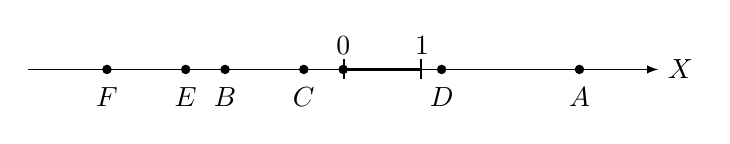
\begin{tikzpicture}[>=latex]
		\draw [fill=black] (0,0) circle(1.5pt);
		\draw [fill=black] (3,0) circle(1.5pt) node[below=3pt]{$A$};
		\draw [fill=black] (-1.5,0) circle(1.5pt)node[below=3pt]{$B$};
		\draw [fill=black] (-.5,0) circle(1.5pt)node[below=3pt]{$C$};
		\draw [fill=black] (1.25,0) circle(1.5pt)node[below=3pt]{$D$};
		\draw [fill=black] (-2,0) circle(1.5pt)node[below=3pt]{$E$};
		\draw [fill=black] (-3,0) circle(1.5pt)node[below=3pt]{$F$};
		
		\draw[->] (-4,0)--(4,0)node [right]{$X$};
		\node at (0,.3){$0$};\node at (1,.3){$1$};
		\draw[thick, |-|](0,0)--(1,0);
		\end{tikzpicture}
		\caption{}
	\end{figure}
\end{solution}

\begin{example}
	把下列各数及它们的相反数都用数轴上的点
	表示出来,并按它们在数轴上从左到右的顺序排列出
	来:
	\[3.5,\quad -2\frac{1}{2} ,\quad 0,\quad -1,\quad +0.5,\quad -\left(-1\frac{1}{2}\right)  \]
\end{example}

\begin{solution}
	所给各数的相反数分别是:
	\[-3.5,\quad +2\frac{1}{2} ,\quad 0,\quad +1,\quad -0.5,\quad -1\frac{1}{2}   \]
	把它们分别用数轴上的点表示为:
	\begin{figure}[htp]
		\centering
		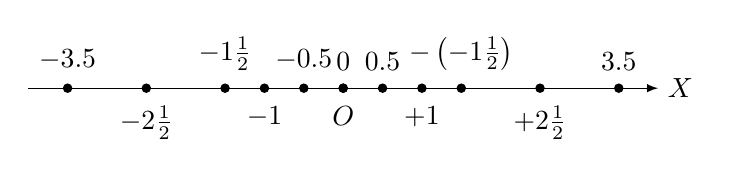
\begin{tikzpicture}[>=latex]
		\draw [fill=black] (0,0) circle(1.5pt) node[below=3pt]{$O$};
		\draw [fill=black] (0,0) circle(1.5pt) node[above=3pt]{$0$};
		\draw [fill=black] (1,0) circle(1.5pt) node[below=3pt]{$+1$};
		\draw [fill=black] (-1,0) circle(1.5pt)node[below=3pt]{$-1$};
		\draw [fill=black] (-.5,0) circle(1.5pt)node[above=3pt]{$-0.5$};
		\draw [fill=black] (.5,0) circle(1.5pt)node[above=3pt]{$0.5$};
		\draw [fill=black] (1.5,0) circle(1.5pt)node[above=3pt]{$-\left(-1\frac{1}{2}\right)$};
		\draw [fill=black] (-1.5,0) circle(1.5pt)node[above=3pt]{$-1\frac{1}{2}$};
		\draw [fill=black] (-3.5,0) circle(1.5pt)node[above=3pt]{$-3.5$};
		\draw [fill=black] (3.5,0) circle(1.5pt)node[above=3pt]{$3.5$};
		\draw [fill=black] (2.5,0) circle(1.5pt) node[below=3pt]{$+2\frac{1}{2}$};
		\draw [fill=black] (-2.5,0) circle(1.5pt)node[below=3pt]{$-2\frac{1}{2}$};
		\draw[->] (-4,0)--(4,0)node [right]{$X$};
		
		\end{tikzpicture}
		\caption{}
	\end{figure}
	
	显然,它们在数轴上从左到右的顺序是:
	\[-3.5,\quad -2\frac{1}{2},\quad -1\frac{1}{2},\quad -1,\quad -0.5,\quad 0,\]
	\[+0.5,\quad +1,\quad +1\frac{1}{2},\quad +2\frac{1}{2},\quad +3.5\]
\end{solution}



从这两个例子可以看出:
\begin{blk}{}
	\begin{itemize}
		\item 正数和负数,确可以表示“相反意义”.说明量的“相反方向”.而数零是它们的界限.
		\item 互为相反的一对数,在数轴上总是表示到
		原点距离相等的一对点.而零与它的相反数都
		用原点表示.
	\end{itemize}    
\end{blk}


既然有理数的正、负号是表示“相反意义”的两
个方向,因此,如果用字母$a$表示一个有理数,那么
它的相反数当然就应该用$-a$表示了.显然,$-a$的相
反数,就可以表示成$-(- a)$,结果自然就有:
$-(-a)=+a$.因为,$-a$的相反数只能是$+a$.

\begin{ex}
	\begin{enumerate}
		\item 试列举出两个正、负有理数来.并写出它们的相反数.同
		时在数轴上标出来.
		\item 如果$a$表示一个负有理数,那么$-a$表示什么数?这两个
		数在数轴上用一对点表示出来后,有什么特征?
		\item 一个有理数$m$,与$(-2)$正好相消,即$(-2)+(m)=0$,
		你知道$m$的值吗?
		\item 如果$(+5) +x=0$,那么$x$应是什么数?
	\end{enumerate}    
\end{ex}    

在一些实际问题中,往往又不考虑“量的方向”,
如:在研究一辆汽车行驶中的耗油量问题中,就只要
计算这辆汽车行驶的里程数,而不需要去追究向什么
方向行驶.这就是说,这种问题中的“路程”,不需
要用“有方向”的正、负数来表示,只要考虑“距
离”.

对于有理数来说,如果仅考虑它在数轴上的点与
原点之间的距离,而不考虑表示这个数的点在原点的
左边还是右边时,我们引入绝对值的概念.

我们规定:\textbf{任一个有理数$a$的绝对值是一个非负
	数},记作$|a|$.

\begin{blk}{}
	\begin{itemize}
		\item 正数的绝对值,就是它本身的值.
		\item 负数的绝对值,就是它的相反数的值.
		\item 零的绝对值,就是0.
	\end{itemize}
\end{blk}

例如:$\left|+2\frac{1}{2}\right|=2\frac{1}{2}$,$|0|=0$,$|-5|=5$,$|-0.7|=0.7$等.

一般地,对任一个有理数$a$,其绝对值可以表示
成:
\[|a|=\begin{cases}
a, & \text{当$a$是正数时}\\
0, & \text{当$a$是0时}\\
-a, & \text{当$a$是负 数时}\\
\end{cases}\]

\begin{ex}
	\begin{enumerate}
		\item (口答)填写下表:
		\begin{center}
			\begin{tabular}{c|cccccc}
				\hline
				$a$ & $+7.2$ & $-\frac{3}{11}$ & 0& $-1012$ &$+1\frac{2}{11}$ &$-1\frac{2}{11}$\\
				\hline
				$|a|$\\
				\hline
			\end{tabular}       
		\end{center}
		\item 如果$|a|=4$,试问:$a$表示何数?
		\item 你能说出“任一对相反数”的绝对值有什么关系吗?并举
		出两例.
	\end{enumerate}
\end{ex}

\section*{习题1.2}
\addcontentsline{toc}{subsection}{习题1.2}
\begin{enumerate}
	\item 用正、负数表示下列各量:
	\begin{enumerate}
		\item 珠穆朗玛峰高出海面8848.13米.
		\item 太平洋最深处低于海面11022米.
		\item 我国新疆吐鲁番盆地低于海面154米.
		\item 北京某地高出海平面47.2米.
	\end{enumerate}
	\item 一座铁桥的长度测量了五次,各次测得的数据是:8015
	米,8009米,8012米,8013米,8011米.
	\begin{enumerate}
		\item 试求这五次测量的平均值.
		\item 如果以“平均值”为基准,试用正、负数表示出各次测量的数值与平均值的差.
	\end{enumerate}
	\item 写出下列各数的相反数:
	\[7,\quad \frac{1}{2},\quad -5,\quad -1\frac{1}{7},\quad 0,\quad 0.7,\quad x,\quad -y  \]
	\item 根据“有理数a的相反数$(- a)$的相反数$-(-a)$
	就是a”的原理,写出下列各式的结果:
	\begin{enumerate}
		\item $-(-2)=\underline{\qquad\qquad}$;
		\item $-\left(-1\frac{1}{4}\right)=\underline{\qquad\qquad}$;
		\item $-[-(0.6)]=\underline{\qquad\qquad}$;
		\item $-[-(-m)]=\underline{\qquad\qquad}$.
	\end{enumerate}
	\item 把下列各数填入应属的集合内:
	\[-5,\quad -\frac{1}{3},\quad 0.34,\quad 0,\quad -1,\quad -3\frac{2}{5},\quad \frac{1}{5},\quad 20\frac{1}{2},\quad -0.001,\quad 10^{10} \]
	\[\text{有理数集合}\begin{cases}
	\text{正有理数集合:}\underline{\qquad\qquad\qquad\qquad\qquad}\\
	\{0\}: \underline{\qquad\qquad\qquad\qquad\qquad}\\    
	\text{负有理数集合:}\underline{\qquad\qquad\qquad\qquad\qquad}\\
	\end{cases}\]
	
	
	\item 在数轴上将下列有理数用点表示出来:
	\begin{enumerate}
		\item $3,\quad -4.1,\quad 1,\quad -\frac{4}{3},\quad 0,\quad 2\frac{1}{2},\quad -1\frac{1}{2}$
		\item $-2.5$的相反数,$0.75$的相反数,0的相反数.
		\item $7500$,$-6250$,$-3750$,$200$.
		(数轴上的单位长要恰当选取,为作图方便,可以取一
		格为1000)
	\end{enumerate}
	
	
	\item 互为相反的一对有理数有什么特征性质?举例说明.
	\item 运用互为相反数的特征,回答下列各题:
	\begin{enumerate}
		\item 如果$(-7) +m=0$,试问:$m$为何数?
		\item 如果$x+\left(3\frac{1}{7}\right)=0$,试问:$x$为何数?
		\item 如果$0+y=0$,试问:$y$为何数?
	\end{enumerate}
	
	
	\item 如果已知有理数$a$与$b$之间有关系“$a+b=0$”,那么,
	你能知道$a$与$b$是什么样的有理数吗?
	\item 写出下列各有理数的绝对值:
	\[-\frac{1}{4},\quad -0.001,\quad 0,\quad +\frac{1}{100},\quad 99\frac{1}{9}\]
	
	\item 如果已知$|x|= 2.7$,那么$x$是什么数?
	\item 在数轴上,到原点的距离等于8个单位长的点,应该
	表示什么有理数?
	\item 填满下列表格:
	\begin{center}
		\begin{tabular}{ccc}
			\hline
			有理数&它的相反数&绝对值\\
			\hline
			$a$  &   $-a$   &   $|a|$\\ 
			$+4$  &   $-4$   &   $4$\\ 
			&   $+0.01$   &   $0.01$\\ 
			&      &   $\frac{1}{6}$\\ 
			$0$  &      &   \\ 
			$-1.2$  &      &   \\ 
			&   $+\frac{8}{9}$   &   \\ 
			&      &   $3\frac{101}{111}$\\ 
			\hline
		\end{tabular}
	\end{center}
	
	\item 填空:
	\begin{enumerate}
		\item 绝对值比5小的整数有(\qquad \qquad ).
		\item 绝对值比4小的负整数有(\qquad \qquad ).
		\item 绝对值比3小的非负整数有(\qquad \qquad ).
		\item 绝对值比6小的自然数有(\qquad \qquad ).
	\end{enumerate}
	
	
	\item 计算:
	\begin{enumerate}
		\item $|0|\x \left|-11\frac{10}{11}\right|+|-0.5|$
		\item $|-4.5|\x\left|+\frac{2^2}{3}\right|$
		\item 已知$(-5)+x=0$,$y+(+25)=0$,试求:$x^2+y$的值.
	\end{enumerate}
	
	\item 你能说出符合下列条件的字母都表示什么样的有理数
	吗?
	\[|a|=a,\qquad |a|=-a,\qquad \frac{|x|}{x}=1,\qquad \frac{|x|}{x}=-1  \]
	
	\item 算一算:
	\begin{enumerate}
		\item $|a|+|-(-a)|-|-a|-|-(-|-a|)|$ ($a$为任一有理数)
		\item $\frac{x}{|x|}-\frac{|x|}{x}$ ($x$是一个非零有理数).
	\end{enumerate}
	
\end{enumerate}

\section{有理数的运算}
引进负数以后,我们就把数的范围扩充到了有理
数系.这样,在应用中就可以统一地处理互为相反意
义的数量问题;在运算上又可以解决在小学算术中减
法“不够减”的矛盾.本节将详细讨论有理数的运算
法则,并运用这些法则进行计算.

这里还要特别指出:我们在提出有理数的各种运
算法则的时候,都是根据相反数的意义及特征性质
$ (-a) + ( + a)=(+a)+(-a) = 0$,并遵从“运算通
性”的要求,首先讨论这些运算法则的合理性,然后,
才去使用这些法则,进行计算.这就是说:引进负数
以后,对于任何有理数的加法、乘法运算,我们仍然
要求它们满足交换律、结合律和分配律,而且,仍然
要求数0与1具有它们原来的运算特性.只有这样,
我们所规定的运算法则,才能是合理的,也只有明确
了这些法则规定是合理的以后,才能进一步应用这些
法则,有效地进行有理数的计算.

\subsection{有理数的加法与减法}
\subsubsection{加法}

在有理数范围内,互为相反数$+a$与$-a$的特征性
质是$(+a) + (-a)=(-a) + (+a) = 0$,反过来说,
假如有一对有理数$a,  b$,它们的总效果$a+b= 0$,我
们就说:$a,  b$互为相反数,即$a=-b$或$b=-a$,显
然,有理数$(a + b)$与$-(a + b)$也是互为相反数.

根据相反数的特征性质,以及要求有理数加法满
足交换律、结合律;要求数0与1仍保持它们在运算
中的特性的原则下,我们首先讨论加法运算法则规定
的合理性,然后再去应用法则.

两个有理数的加法运算,可分三种情形讨论如
下:设$a,  b$分别是正值.
\begin{enumerate}
	\item 两个正有理数相加,即$(+ a)+(+b)$.
	\item 两个负有理数相加,即$(-a)+(-b)$.
	\item 一个正有理数与一个负有理数相加,即
	$(+a)+(-b)$
\end{enumerate}

很显然,在1的情形,就是小学算术中的加
法.即
\[(+a)+(+b)=+(a+b)\]

例如:某单位收入五万元,后又收入2万元;显然一
共收入应是7万元,即:$(+5)+(+2)=+7$

在情形2,我们可以根据相反数的特性及运
算通性继续有效来讨论:由于
\begin{align*}
&\quad (-a) +(-b) + (+a) + (+b)\\
&=[(-a)+(+a)]+[(-b)+(+b)]
\tag{加法交换、结合律}\\
&=0+0\tag{相反数的特性}\\
&=0\tag{零的运算}
\end{align*}
而且,由加法运算的情形1知道,
\[(+a)+(+b)=+(a+b)\]

所以$( - a) + (- b) + (a + b) = 0$.
这就是说,$( - a)$与
$(-b)$的和,应等于$(a + b)$的相反数.

因此,我们规定:
\[(-a)+(-b)=-(a+b)\]

这样规定,既是合理的,也是符合实际的,例
如:某家公司,今年亏损2.5万元,而去年已经亏损
3万元,两年共亏损5.5万元.即:
\[(-2. 5)+(-3)=-(2.5+3)=-5.5\; (\text{万元})\]
综合情形1、2,可以得出:
\begin{blk}{}
	符号相同的两个有理数相加,只要将两数的绝对
	值相加,符号仍取原来的符号就行了.
\end{blk}

对于情形3:$(+a)+(-b)$,我们还需要根
据$a,b$(实际上就是$+a$,$-b$的绝对值)的大小分别讨
论.

例如:
\begin{align*}
(+5)+(-3)&=(+2+3)+(-3)\\
&=(5-3 + 3)+(-3)\\
&=+(5-3)+[(+3)+(-3)]\tag{加法结合律}\\
&=+(5-3)+0 \tag{相反数的性质}\\
&=+(5-3)\tag{零的特性}\\
\end{align*}

一般地:当$a$大于$b$时,
\begin{align*}
(+ a)+(-b)&=+(a-b + b)+(-b)\\
&=+(a-b)+[(+b)+(-b)]    \tag{加法结合律}\\
& =+(a-b) + 0 \tag{零的特性}\\
&  =+(a-b)
\end{align*}

所以,在$a$大于$b$时,我们规定:
\[(+a)+(-b)=+(a-b),\qquad (\text{$a$大于$b$时})\]
这个规定也是符合实际的,比如:温度计上升10\oc,
又下降8\oc,其结果显然是上升2\oc,即:
\[     (+10)+(-8)=+(10-8)=+2\]

同样,当$a$小于$b$时,我们可以作类似讨论:
\begin{align*}
(+ a)+(-b)&=(+ a)+[-(b-a+a)]\\
& =(+ a)+[-(b-a)+( -a)]   \tag{情形2加法法则}\\
&=[(+ a)+(-a)]+[-(b-a) ]  \tag{加法交换、结合律}\\
&=0+[-(b-a)]\tag{相反数的特性}\\
&=-(b-a)\tag{零的特性}\\
\end{align*}


所以,在$a$小于$b$时,我们规定:
\[(+a)+(-b)=-(b-a),\qquad (\text{$a$小于$b$时})\]
这样规定,同样是符合实际的,比如:气温上升10.5\oc,
接着又下降12\oc,其结果自然应该是下降1.5\oc,即
\[(+10.5)+(-12)=-(12-10.5)=-1.5\]

综合对情形3的讨论,可以得出:
\[(+a)+(-b)=\begin{cases}
+(a-b),& (\text{$a$大于$b$时})\\
-(b-a),& (\text{$a$小于$b$时})
\end{cases}\]
这就是说:

\begin{blk}{}
	两个符号相反的有理数相加,只要将较大的绝对
	值减去较小的绝对值,符号取绝对值较大的加数的符
	号就行了.
\end{blk}

\begin{example}
	运用加法法则,计算下列各题:
	\begin{multicols}{2}
		\begin{enumerate}
			\item $(+8)+\left(+1\frac{1}{2}\right)$;
			\item $(+5.02)+\left(+0.98\right)$;
			\item $(-10.1)+\left(-\frac{9}{10}\right)$;
			\item $\left(-1\frac{1}{3}\right)+\left(-2\frac{1}{4}\right)$;
			\item $(+99)+(-79)$;
			\item $(-101)+(+100.9)$;
			\item $(+57\frac{1}{3})+\left(-57\frac{1}{2}\right)$;
			\item $\left(+1\frac{1}{9}\right)+\left(-4\frac{1}{90}\right)$.
		\end{enumerate}
	\end{multicols}
\end{example}    

\begin{solution}
	\begin{enumerate}
		\item $(+8)+\left(+1\frac{1}{2}\right)=+\left(8+1\frac{1}{2}\right)=+9\frac{1}{2}$
		\item $(+5.02)+\left(+0.98\right)=+6$
		\item $(-10.1)+\left(-\frac{9}{10}\right)=-\left(10.1+\frac{9}{10}\right)=-(10.1+0.9)=-11$
		\item $\left(-1\frac{1}{3}\right)+\left(-2\frac{1}{4}\right)=-\left(1\frac{1}{3}+2\frac{1}{4}\right)=-\left(\frac{16}{12}+\frac{27}{12}\right)=-\frac{43}{12}=-3\frac{7}{12}$
		\item $(+99)+(-79)=+(99-79)=+20$
		\item $(-101)+(+100.9)=-(101-100.9)=-0.1$
		\item $(+57\frac{1}{3})+\left(-57\frac{1}{2}\right)=-\left(57\frac{1}{2}-57\frac{1}{3}\right)=-\frac{1}{6}$
		\item $\left(+1\frac{1}{9}\right)+\left(-4\frac{1}{90}\right)=-\left(4\frac{1}{90}-1\frac{1}{9}\right)=-2\frac{81}{90}=-2\frac{9}{10}$
		
	\end{enumerate}
	
\end{solution}

\begin{example}
	计算:
	\begin{enumerate}
		\item $(+2)+(-4)+(-8)$;
		\item $\left(-\frac{2}{3}\right)+\left(+\frac{4}{5}\right)+\left(-\frac{1}{3}\right)+\left(+1\frac{1}{5}\right)$;
		\item $(-x)+(-y)+x$;
		\item $(-a)+(-a)$.
	\end{enumerate}
\end{example}

\begin{analyze}
	遇到三个以上有理数相加时,可以按照
	运算顺序从左到右逐次相加(运用结合律);也可以
	运用交换律、结合律将同号各数分别结合在一起相
	加,再求总结果.
\end{analyze}


\begin{solution}
	\begin{align*}
	(+2)+(-4)+(-8)&= [(+2)+(-4)]+(-8) \tag{结合律}\\
	&=(-2)+(-8) \tag{异号相加法则}\\
	&=-10 \tag{同号相加法则}
	\end{align*}
	
	\begin{align*}
	&\quad   \left(-\frac{2}{3}\right)+\left(+\frac{4}{5}\right)+\left(-\frac{1}{3}\right)+\left(+1\frac{1}{5}\right)\\
	&=\left[\left(-\frac{2}{3}\right)+\left(-\frac{1}{3}\right)\right]+\left[\left(+\frac{4}{5}\right)+\left(+1\frac{1}{5}\right)\right]  \tag{交换、结合律}\\
	&=-\left(\frac{2}{3}+\frac{1}{3}\right)+\left[+\left(\frac{4}{5}+1\frac{1}{5}\right)\right]  \tag{同号加法法则}\\
	&=(-1)+(+2)=+1  \tag{异号加法法则}
	\end{align*}
	
	\begin{align*}
	(-x)+(-y)+x  &= [(-x)+x]+(-y)  \tag{交换、结合律}\\
	&=0+(-y) \tag{相反数的性质}\\
	&=-y \tag{零的特性}
	\end{align*}
	
	\begin{align*}
	(-a)+(-a) &= (-1)a+(-1)a  \tag{相反数的意义}\\
	&=[(-1)+(-1)]a  \tag{分配律}\\
	&=-2a  \tag{同号加法法则}\\
	\end{align*}
\end{solution}

总起来说,有理数加法法则是:

\begin{blk}{有理数加法法则}
	\begin{enumerate}
		\item 同号相加:
		\[\begin{split}
		(+a)+(+b)&=+(a+b)\\
		(-a)+(-b)&=-(a+b)
		\end{split}\]
		\item 异号相加:
		\[(+a)+(-b)=\begin{cases}
		+(a+b),& a>b\\
		-(b-a),&a<b
		\end{cases}\]
		\item 相反数相加:
		\[(+a)+(-a)=0\]
		\item 与零相加:
		\[\begin{split}
		(+a)+0&=0+(+a)=+a\\
		(-a)+0&=0+(-a)=-a\\
		0+0&=0
		\end{split}\]
	\end{enumerate}    
	其中的$a,b$都是正数.
\end{blk}

\begin{ex}
	\begin{enumerate}
		\item (口答)计算:
		\[(+7)+(-5),\qquad (-7)+(+5),\qquad (-7)+(-5) \]
		\[\left(+\frac{1}{3}\right)+\left(+\frac{1}{2}\right),\; \left(+\frac{1}{3}\right)+\left(-\frac{1}{2}\right),\; \left(-\frac{1}{3}\right)+\left(+\frac{1}{2}\right) ,\; \left(-\frac{1}{3}\right)+\left(-\frac{1}{2}\right) \]
		\[(+0.8)+(-1.6),\; (-0.8)+(-1.6),\; (-0.8)+(+1.6),\; (+0.8)+(+1.6) \]
		\[2+\left(-1\frac{1}{5}\right),\;\;(-2)+\left(-1\frac{1}{5}\right),\;\;(-2)+\left(+1\frac{1}{5}\right),\;\; 0+\left(-1\frac{1}{5}\right)\]
		\item 计算:
		\[1+\left(-\frac{1}{2}\right)+\left(-\frac{1}{3}\right)+\left(-\frac{1}{6}\right),\qquad \left(-\frac{1}{5}\right)+0+\left(+\frac{8}{15}\right)+\left(-\frac{4}{15}\right) \]
		\[\left(-1\frac{1}{3}\right)+\left(+\frac{2}{3}\right)+0+\left(-\frac{2}{3}\right)+\left(+\frac{4}{3}\right),\qquad a+a+(-a) \]
	\end{enumerate}
\end{ex}

\subsubsection{减法}

减法是加法的\textbf{逆运算}.比如$(-5)-(+3)$的问
题,就是要求一个数$[?]$,使得$[?]+(+3)=(-5)$.
也就是说,$(-5)-(+ 3)$是一个数$[?]$,这个数能
够使得$[?]+(+3)=(-5)$成立.即
$$[(-5)-(+3) ]+(+3)=(-5)$$

但我们由有理数加法法则可以知道,只有
\[(-8)+(+3)=-5\]
显然得出:
\begin{equation}
(-5)-(+3)=-8
\end{equation}

又由加法可知:
\begin{equation}
(-5)+(-3)=-8
\end{equation}

比较(1.1)、(1.2)两式,不难得出:
\[ (-5)-(+3)=(-5)+(-3)=-8\]
这就是说:有理数$(-5)$减去$(+ 3)$,就等于$(-5)$
加上$(+ 3)$的\textbf{相反数}$(-3)$.减法就转化成了加法
计算.

同样地,$\because\quad (+3)+(-7)=-4$
\begin{equation}
\therefore\quad    (-4)-(-7)=+3
\end{equation}    
又由加法可知:
\begin{equation}
(-4)+(+7)=+3
\end{equation}
比较(1.3)、(1.4)两式,又可以得出:
\[ (-4)-(-7)= (-4)+(+7)=+3\]
即,$(-4)$\textbf{减}去$(-7)$就等于$(-4)$\textbf{加}上$(-7)$
的\textbf{相反数}$(+7)$.这里又把减法转化为加法了.

由此,可以归纳出\textbf{有理数减法的法则是:}

\textbf{减去一个有理数,就等于加上这个有理数的相反
	数}.若用宇母表示有理数,则有理数$x$,$y$的减法法
则是:

\begin{center}
	\begin{tikzpicture}[>=latex]
	\node at (0,0) {\LARGE $ x-y=x+(-y)$}  ;
	\draw[dashed, <->] (-1.5,.3)--(-1.5,1)--node[above]{减法化加法}(.7,1)--(.7,.3);
	\draw[dashed, <->] (-1,-.3)--(-1,-1)--node[below]{换成相反数}(2,-1)--(2,-.3);
	\end{tikzpicture}
\end{center}

\begin{example}
	利用减法法则,计算下列各题:
	\begin{multicols}{2}
		\begin{enumerate}
			\item $(+9)-(-5)$
			\item $\left(-\frac{3}{4}\right)-\left(+\frac{1}{2}\right)$
			\item $(+0.7)-(-0.21)$
			\item $0-(+8)$
			\item $(-5)-0$
			\item $(-2.7)-(+5)$
			\item $\left(-1\frac{1}{2}\right)-\left(-\frac{1}{3}\right)$
			\item $(-a)-(-a)$
		\end{enumerate}
	\end{multicols}
\end{example}

\begin{solution}
	\begin{enumerate}
		\item $(+9)-(-5)=(+9)+(+5)=+14$
		\item $\left(-\frac{3}{4}\right)-\left(+\frac{1}{2}\right)=\left(-\frac{3}{4}\right)+\left(-\frac{1}{2}\right)=-\left(\frac{3}{4}+\frac{1}{2}\right)=-\frac{5}{4}=-1\frac{1}{4}$
		\item $(+0.7)-(-0.21)=(+0.7)+(+0.21)=+0.91$
		\item $0-(+8)=0+(-8)=-8$
		\item $(-5)-0=(-5)+0=-5$
		\item $(-2.7)-(+5)=(-2.7)+(-5)=-7.7$
		\item $\left(-1\frac{1}{2}\right)-\left(-\frac{1}{3}\right)=\left(-1\frac{1}{2}\right)+\left(+\frac{1}{3}\right)=-\left(\frac{3}{2}-\frac{1}{3}\right)=-\frac{7}{6}$
		\item $(-a)-(-a)=(-a)+(+a)=0$
	\end{enumerate}    
\end{solution}

\begin{example}
	计算:
	\begin{enumerate}
		\item $(+1)-\left(-\frac{1}{2}\right)-\left(-\frac{1}{3}\right)-\left(-\frac{1}{6}\right)$
		\item $(+1)-\left(+\frac{1}{2}\right)-\left(+\frac{1}{3}\right)-\left(+\frac{1}{6}\right)$
		\item $(-b)-(+b)-(-b)-(+a)$
	\end{enumerate}
\end{example}

\begin{analyze}
	遇到几个有理数连减时,仍可从左到右
	按顺序逐次相减——也就是逐次加上各数的相反数.
\end{analyze}

\begin{solution}
	\begin{align*}
	&\quad   (+1)-\left(-\frac{1}{2}\right)-\left(-\frac{1}{3}\right)-\left(-\frac{1}{6}\right)\\
	&= (+1)+\left(+\frac{1}{2}\right)+\left(+\frac{1}{3}\right)+\left(+\frac{1}{6}\right)\tag{减法法则}\\
	&=(+1)+\left(\frac{1}{2}+\frac{1}{3}+\frac{1}{6}\right)\tag{同号相加法则}\\
	&=+2
	\end{align*}   
	
	\begin{align*}
	&\quad    (+1)-\left(+\frac{1}{2}\right)-\left(+\frac{1}{3}\right)-\left(+\frac{1}{6}\right)\\
	&=(+1)+\left(-\frac{1}{2}\right)-\left(+\frac{1}{3}\right)+\left(-\frac{1}{6}\right)\tag{减法法则}\\
	&=(+1)+\left[ \left(-\frac{1}{2}\right)+\left(-\frac{1}{3}\right) +\left(-\frac{1}{6}\right)\right]  \tag{加法结合律}\\
	&=(+1)+\left[-\left(\frac{1}{2}+\frac{1}{3}+\frac{1}{6}\right)\right]\tag{同号相加法则}  \\
	&=(+1)+(-1)=0  \tag{相反数性质}
	\end{align*}   
	
	\begin{align*}
	(-b)-(+b)-(-b)-(+a)&=(-b)+(-b)+(+b)+(-a)\tag{减法法则}\\
	&=(-b)+[(-b)+(+b)]+(-a)  \tag{加法结合律}\\
	&=(-b)+0+(-a) \tag{相反数意义}\\
	&=(-b)+(-a) \tag{零的特征}\\
	&=-(a+b)  \tag{同号相加法则}    
	\end{align*}   
\end{solution}

\begin{ex}
	\begin{enumerate}
		\item 口答下列各题:
		\[(+3)-(+5),\quad (+3)-(-5),\quad (-3)-(+5),\quad (-3)-(-5) \]
		\[(+5)-(+2.5),\quad  (+5)-(-2.5),\quad (-5)-(-2.5),\quad (-5)-(+2.5)\]
		\[\left(-7\frac{1}{2}\right)-\left(-7\frac{1}{2}\right),\;\; \left(-7\frac{1}{2}\right)-\left(+7\frac{1}{2}\right),\;\; \left(-7\frac{1}{2}\right)-0,\;\; 0-\left(-7\frac{1}{2}\right) \]
		\[(-a)-(+a),\quad (-a)-(-a),\quad (+a)-(-a),\quad 0-(-a)\]
		
		\item 计算:
		\begin{enumerate}
			\item $(+2.1)-(-0.9)-1$
			\item $(-2.1)-(-0.9)-0-(+7)$
			\item $\left(-1\frac{1}{5}\right)-\left(-\frac{3}{5}\right)-\left(+\frac{1}{5}\right)$
			\item $(+a)-(0.625)-(+0.025)-(-0.415)-(+0.015)-(-a)$
		\end{enumerate}
	\end{enumerate}  
\end{ex}

通过有理数减法的学习,我们就进一步明确了:
引进负数后,“不够减”的矛盾就解决了,\textbf{在有理数
	范围内,减法运算也是畅通无阻的}.


\subsection{代数和}
有理数的减法运算都可以转化为加法进行,这样
一来,在有理数范围内,“求和”与“求差”的问题
就可以统一称为“求和”的问题了.比如:

算式$(+ 3)+(-7)-(-5)+(+9)-(+2)$中,
只有加、减运算,利用减法法则就可以统一写成“求
和”的式子:
\begin{equation}
(+ 3)+(-7)+(+5)+(+9)+(-2)
\end{equation}

象这样,含有加、减法运算的式子,都能转化成
仅含有加法运算的式子,我们称作“代数和”.式
(1.5)就是代数和.

在代数和中,被加号“+”隔开的每一部分,叫
做一项,如式(1.5)中,$(+3)$, $(-7)$, $(+ 5)$,
$(+9)$, $(-2)$都是代数和(1.5)的一项.

求各项的代数和,就是对各项进行加法运算.

在计算两项以上的代数和时,有效地应用加法的
交换律、结合律,先将所有的正数项、所有的负数项
分别求和,再将这两部分相加求其总和,可以使计算
大为简便.

\begin{example}
	计算:$(+3)+(-7)+(+5)+(+9)+(-2)+(-8)$
\end{example}

\begin{solution}
	\begin{align*}
	\text{原式}&= [(+3)+(+5)+(+9)]+[(-7)+(-2)+(-8)] \tag{交换、结合律}\\
	&=(+17)+(-17) \tag{同号加法法则}\\
	&=0 \tag{相反数的特性}
	\end{align*}
\end{solution}

\begin{example}
	计算:$(-6.5)-(-7.3)-(-3.7)+(-12.5)-\left(-\frac{1}{2}\right)$
\end{example}

\begin{solution}
	\begin{align*}
	\text{原式}&= (-6.5)+(+7.3)+(+3.7)+(-12.5)+\left(+\frac{1}{2}\right) \tag{减法法则}\\
	&=[(-6.5)+(-12.5)]+\left[(+7.3)+(+3.7)+\left(+\frac{1}{2}\right)\right] \tag{交换、结合律}\\
	&=(-19)+\left(+11\frac{1}{2}\right) \tag{同号相加法则}\\
	&=-7\frac{1}{2} \tag{异号相加法则}
	\end{align*}
\end{solution}

在代数和式子中,经常省去各项之间的加号“$+$”
及第一项前的正号“$+$”.比如例1.21中的代数和,可
以写成:$3-7+5+9-2$.读作:“正3负7正5正
9负2的和.”或者读成:“3减7加5加9减2”.

同样,
例1.22中的代数和,可以写成:$-6.5+7.3+3.7-12.5+\frac{1}{2}$
读作:“负6.5正7.3正3.7负12.5正$\frac{1}{2}$的和”.或者读成:“负6.5加7.3加3.7减12.5
加$\frac{1}{2}$”.




\begin{example}
	计算代数和:
	\[\left(+\frac{3}{4}\right)+\left(+\frac{1}{2}\right)+\left(-\frac{3}{8}\right)+\left(-\frac{1}{4}\right)+\left(-\frac{1}{8}\right)  \]   
\end{example}


\begin{solution}
	\begin{align*}
	\text{原式}&=\frac{3}{4}+\frac{1}{2}-\frac{3}{8}-\frac{1}{4}-\frac{1}{8}  \tag{简化代数和}\\
	&=\left(\frac{3}{4}+\frac{1}{2}\right)-\left(\frac{3}{8}+\frac{1}{4}+\frac{1}{8}\right)\\
	&=\frac{5}{4}-\frac{6}{8}=\frac{2}{4}=\frac{1}{2}
	\end{align*}  
\end{solution}

\begin{ex}
	计算代数和:
	\begin{enumerate}
		\item $0+(-24)+(-5)+7$
		\item $-7.2-0.9-5.6+1.7$
		\item $13\frac{4}{5}+0-2\frac{2}{5}-8-6\frac{1}{5}$
		\item $-\frac{7}{5}-1\frac{1}{5}-2\frac{3}{5}+3\frac{1}{5}+2-\frac{4}{5}+a$
	\end{enumerate} 
\end{ex}

\begin{example}
	设有有理数$a,b,c,d$,说明等式:$a-b+c-d=a-(b-c+d)$成立.
\end{example}

\begin{solution}
	\begin{align*}
	a-b+c-d&= a+(-b)+c+(-d) \tag{代数和原意}\\
	&=a+ (-1)\cdot b+(-1)\cdot (-c)+(-1)\cdot d  \tag{相反数意义}\\
	&=a+(-1)(b-c+d) \tag{分配律}\\
	&=a-(b-c+d)  \tag{相反数意义}    
	\end{align*}    
	$\therefore\quad a-b+c-d=a-(b-c+d)$
\end{solution}

这就告诉我们:在计算代数和,遇到需要添加或
去掉括号时,要遵守这样的规则:

\begin{blk}{}
	在紧接负号后边添加括号时,括到括号里的每一
	项,都要改变符号;而要脱掉紧接负号后边的括号
	时,又必须将括号与紧接括号前边的负号都去掉,并
	将原括号内的各项都改变符号.
\end{blk}



\begin{example}
	计算:
	\begin{enumerate}
		\item $2-\frac{1}{2}-\frac{1}{3}-\frac{1}{6}$
		\item $-1\frac{3}{4}-\left[\frac{1}{2}-\left(\frac{3}{4}+\frac{1}{2}-1\frac{3}{8}\right)+\frac{5}{8}\right]$
	\end{enumerate}
\end{example}

\begin{solution}
	可以灵活运用添、去括号的规则进行计算.
	\[ \begin{split}
	2-\frac{1}{2}-\frac{1}{3}-\frac{1}{6}&=2-\left(\frac{1}{2}+\frac{1}{3}+\frac{1}{6}\right)\\
	&=2-1=1
	\end{split}  \]
	\[ \begin{split}
	&\quad -1\frac{3}{4}-\left[\frac{1}{2}-\left(\frac{3}{4}+\frac{1}{2}-1\frac{3}{8}\right)+\frac{5}{8}\right]\\
	&=-1\frac{3}{4}-\left[\frac{1}{2}-\frac{3}{4}-\frac{1}{2}+1\frac{3}{8}+\frac{5}{8}\right]\\
	&=-\frac{7}{4}-\bcancel{\frac{1}{2}}+\frac{3}{4}+\bcancel{\frac{1}{2}}-\frac{11}{8}-\frac{5}{8}\\
	&=-\frac{4}{4}-\frac{16}{8}\\
	&=-1-2=-3
	\end{split}  \]
\end{solution}

\begin{ex}
	\begin{enumerate}
		\item 先转化为加法,再计算:
		\begin{enumerate}
			\item $\left(3\frac{1}{3}\right)^2-\left(+\frac{5}{6}\right)-\left(1\frac{1}{4}\right)^2$
			\item $\left(-5\frac{7}{12}\right)+\left(-1\frac{3}{4}\right)-\left(-1\frac{1}{4}\right)+5\frac{7}{12}-27$
		\end{enumerate}
		\item 计算代数和:
		\begin{enumerate}
			\item $27.5-\left(-1-\frac{3}{7}-5\right)+\frac{4}{7}$;
			\item $-1.5-[1.4-(-3.6)-4.3+(-5.2)]$.
		\end{enumerate}
		\item 在括号内填上适当的项,使等式成立:
		\[a+b-c+d=a+b-(\qquad \qquad )\]
		\[ a-b+c+d=a-(\qquad \qquad )     \]
	\end{enumerate}    
\end{ex}

\subsection{有理数的乘法与除法}

对于有理数的乘法和除法,我们仍然是根据相反
数的特征性质$(-a)+(+a)=0$,以及要使“运算通
性”(指加、乘法满足交换、结合和分配律;数0与
1仍有原先的运算特性)继续有效的原则下,我们去
讨论它的运算法则如何规定才合理?在此基础上,再
去进一步学习和运用这些法则进行计算.

\subsubsection{乘法}
两个有理数的乘法运算,仍可分为三种情形进行
讨论:仍设$a,  b$是两个正有理数.
\begin{enumerate}
	\item 两个正有理数相乘,即$(+a) \x (+ b)$;
	\item 一个正,一个负有理数相乘,即$(+a) \x
	(-b)$;
	\item 两个负有理数相乘,即$(-a) \x(-b)$.
\end{enumerate}

对于情形1,很显然,两个正有理数相乘,
就是与小学算术中所学乘法是一样的,即
\[(+a)\x (+b)=ab \]
例如:$\left(+\frac{1}{3}\right)\x \left(+\frac{2}{5}\right)=\frac{1}{3}\x \frac{2}{5}=\frac{2}{15}$

对于情形2,我们作以下的讨论:

由于$(+ b) +(-b)= 0$以及$(+a) \x (+b) =ab$
已经知道,再利用我们约定应该继续有效的“数系运
算通性”,就可以得出:
\begin{align*}
(+a) \x (+b) +(+a) \x (-b) &=(+a)[(+b)+(-b)] \tag{分配律}\\
&=(+a)\x 0  \tag{相反数的特性}\\
&=0 \tag{零的特性}
\end{align*}

这就是说,$ab +(+ a) \x(-b)=0$.

可见,$(+a) \x (-b)$的积与$ab$应是互为相反
数,因而,我们就应该规定:
\[(+a)\x (-b)=-ab \]

同样的讨论,可以得出:\[(-a)\x (+b)=-ab \]

又由于,要使乘法运算满足交换律,就应该有以
下合理的规定:
\[\begin{split}
(+a) \x(-b)&=(-b) \x(+ a)\\
&=(-a) \x(+ b)\\
&=(+ b) \x(-a)=-ab
\end{split}\]

所以,\textbf{两异号(一负一正)有理数相乘,将绝对
	值相乘,符号取负.}

例如:$a\x(-2)=-2a$
\[(+5)\x \left(-\frac{3}{5}\right)=-\left(5\x \frac{3}{5}\right)=-3  \]
\[(-2)\x \left(+\frac{1}{3}\right)=2\x \left(-\frac{1}{3}\right)=-\frac{2}{3} \]


对于情形3,两个负有理数相乘,我们也可
以作类似讨论:
\begin{align*}
&\quad   (+ a) \x(-b)+(-a) \x(-b)\\
& =[(+ a)+(-a) ] \x(-b) \tag{分配律}\\
&=0\x(-b) \tag{相反数的特性}\\
& =0   \tag{零的特性}
\end{align*}
即:$(+ a) \x(-b)+(-a) \x(-b)=0$.

也就是说,$- ab$与$(-a) \x(-b)$应是互为相反
数,因而乘积$(-a) \x(-b)$就是$-(-ab)=+ ab$.

所以,两个负有理数相乘时,应该规定:
\[(-a)\x (-b)=+ab \]

这就告诉我们:\textbf{两个负有理数相乘,将绝对值相
	乘,符号取正.}

例如:$(-b)\x(-3)=+(b\x 3)=+3b$
$$\left(-\frac{3}{4}\right)\x\left(-\frac{1}{2}\right)=+\left(\frac{3}{4}\x \frac{1}{2}\right)=+\frac{3}{8}$$

综合情形1、2、3,可得到两个
非零有理数的乘法法则:\textbf{将绝对值相乘,而积的符号
	是:同号得正,异号得负.}
再加上我们一开始就约定继续有效的
“零的运算特性”:
\[\begin{split}
(+a)\x 0&=0\x (+a)=0\\
(-a)\x 0&=0\x (-a)=0\\
0\x 0&=0
\end{split}\]
这样,对任意两个有理数都可以进行乘法运算了.

\begin{example}
	计算下列各题:
	\begin{enumerate}
		\item $(+7)\x (+10),\quad (-7)\x (+10),\quad (+7)\x (-10),\quad (-7)\x (-10)$
		\item $(-0.5)\x (+0.4),\qquad (-0.5)\x (-0.4)$
		\item $(-a)\x (-1),\quad (-a)\x (-2),\quad (-a)\x (+5),\quad (-a)\x 0$
		\item $\left(-\frac{3}{7}\right)\x \left(+1\frac{1}{6}\right),\qquad \left(-\frac{3}{7}\right)\x \left(-1\frac{1}{6}\right)$
		\item $(+1.5)\x \left(-2\frac{2}{3}\right),\quad (-1.5)\x \left(-2\frac{2}{3}\right),\quad (-1.5)\x \left(-\frac{101}{111}\right)\x 0$
	\end{enumerate}
	
\end{example}

\begin{solution}
	\begin{enumerate}
		\item $(+7)\x (+10)=70,\qquad (-7)\x (+10)=-70$ 
		\[(+7)\x (-10)=-70,\qquad (-7)\x (-10)=70\]
		\item $(-0.5)\x (+0.4)=-0.2,\qquad (-0.5)\x (-0.4)=0.2$
		\item $(-a)\x (-1)=a,\qquad (-a)\x (-2)=2a$  $$(-a)\x (+5)=-5a,\qquad (-a)\x 0=0$$
		\item $\left(-\frac{3}{7}\right)\x \left(+1\frac{1}{6}\right)=-\left(\frac{3}{7}\x\frac{7}{6}\right)=-\frac{1}{2},\qquad \left(-\frac{3}{7}\right)\x \left(-1\frac{1}{6}\right)=\frac{1}{2} $
		\item  $(+1.5)\x \left(-2\frac{2}{3}\right)=-\left(\frac{3}{2}\x\frac{8}{3}\right)=-4$
		\[(-1.5)\x \left(-2\frac{2}{3}\right)=4,\qquad (-1.5)\x \left(-\frac{101}{111}\right)\x 0=0 \]
	\end{enumerate}
	
\end{solution}  

\begin{example}
	计算:
	\begin{enumerate}
		\item $(-7) \cdot(+3) \cdot(+5) \cdot(-2) \cdot\left(-\frac{1}{21}\right)$
		\item 
		$(+0.1) \cdot(-2.5) \cdot(+4) \cdot(-9) \cdot(+100)$
	\end{enumerate}
\end{example}

\begin{analyze}
	求两个以上有理数的乘积时,一般应按
	顺序从左到右两两逐个计算,但,利用乘法的交换、
	结合律,可以简化计算.
\end{analyze}

\begin{solution}
	\begin{align*}
	&\quad   (-7) \cdot(+3) \cdot(+5) \cdot(-2) \cdot\left(-\frac{1}{21}\right)\\
	&=\left[(-7)\cdot (+3)\cdot \left(-\frac{1}{21}\right)\right]\cdot [(+5)\cdot (-2)]\tag{交换、结合律}\\
	&=\left[(-21)\cdot \left(-\frac{1}{21}\right)\right]\cdot [(-10)] \tag{异号相乘法则}\\
	&=(+1)\cdot (-10) \tag{同号相乘法则}\\
	&=-10 \tag{1的特性}
	\end{align*} 
	\begin{align*}
	&\quad (+0.1) \cdot(-2.5) \cdot(+4) \cdot(-9) \cdot(+100)\\
	&=[(+0.1)\cdot (+100)\cdot(-9)]\cdot[(-2.5)\cdot (+4)]\\
	&=(-90)\cdot (-10)=+900
	\end{align*}    
\end{solution}

从例1.27两题的计算结果中,你能发现“几个非零
有理数连乘时,乘积的符号与负乘数的个数之间”有
什么规律吗?

再观察两个例子:
\[(-1)\cdot (-2)\cdot (+3)\cdot \left(-\frac{1}{2}\right)\cdot \left(-\frac{1}{3}\right)=+1  \]
\[(-1)\cdot (-2)\cdot (-3)\cdot \left(-\frac{1}{2}\right)\cdot \left(-\frac{1}{3}\right)=-1  \]

可见,在计算若干个非零有理数的连乘积时,只
要将绝对值相乘,而乘积的符号,可以直接由“负乘
数的个数”来确定,即:

\begin{blk}{}
	当负乘数有奇数个时,乘积为负;
	
	当负乘数有偶数个时,乘积为正.
\end{blk}

显然,若干个有理数相乘,如果其中只要\textbf{有一个}
乘数\textbf{为零},那么,根据零的特性,就知道所得乘积必
定是\textbf{零},就不必再去逐一计算了.


\begin{example}
	计算:
	\begin{enumerate}
		\item $\left(-1 \frac{1}{2}\right) \cdot\left(+\frac{2}{3}\right) \cdot\left(-\frac{7}{10}\right)\cdot\left(-1 \frac{4}{7}\right) \cdot\left(+2 \frac{1}{5}\right)$
		\item $\left(-\frac{273}{113}\right) \cdot\left(+99 \frac{19}{100}\right)\cdot\left[7 \frac{1}{8}+\left(-7 \frac{1}{8}\right)\right] \cdot\left(-29^{2}\right)$
		\item $2 \cdot(-a) \cdot(-5) \cdot(-b)$
	\end{enumerate}
\end{example}

\begin{solution}
	\begin{enumerate}
		\item 原式中含有三个(奇数个)负乘数,因而其乘积为负.
		\[\begin{split}
		\text{原式}&=-\left(1\frac{1}{2}\x\frac{2}{3}\x\frac{7}{10}\x1\frac{4}{7}\x2\frac{1}{5}\right)\\
		&=-\frac{121}{50}=-2\frac{21}{50}
		\end{split}\]
		\item $\text{原式}=\left(-\frac{273}{113}\right) \cdot\left(+99 \frac{19}{100}\right)\cdot 0 \cdot\left(-29^{2}\right)=0$
		\item $2 \cdot(-a) \cdot(-5) \cdot(-b)=-10ab$
	\end{enumerate}
\end{solution}

这里要指出,对于含有字母的算式,计算中只要
注意字母前所带的正、负号就可以,不必去讨论字母
本身是正数还是负数.

\begin{ex}
	\begin{enumerate}
		\item 口答:
		\[(-2)\cdot (+15),\quad (-2)\cdot (-15),\quad -(-2)\cdot (-15),\quad -(+2)\cdot (-15)\]
		\[(-0.25)\cdot (+8),\quad (-0.25)\cdot (-8),\quad -(+0.25)\cdot (-8),\quad(-0.25)\cdot [-(-8)] \]
		\[(-1981)\cdot 0,\qquad 0\cdot\left(+11\frac{1}{22}\right)\]
		\[\left(-\frac{4}{7}\right)\cdot \left(+1\frac{3}{4}\right),\quad \left(-1\frac{3}{4}\right)\cdot\left(-\frac{4}{7}\right),\quad -\left(-1\frac{3}{4}\right)\cdot\left(+\frac{4}{7}\right)\]
		
		\item 计算:
		\begin{enumerate}
			\item $(-1)\cdot(+1)\cdot (-1949)\cdot (-1)$
			\item $(-3)\cdot \left(+\frac{5}{6}\right)\cdot \left(-1\frac{4}{5}\right)\cdot\left(-\frac{1}{4}\right)$
			\item $(-0.25)\cdot (-1.25)\cdot (+4)\cdot (-8)\cdot (+2000)\cdot (-0.001)$
			\item $[(-9)+(+7)-13]\cdot [4+(-7)]\cdot 9$
			\item $\left(-\frac{3}{4}\right)\cdot \left(-8+\frac{2}{3}-1\frac{1}{3}\right)$
			\item $(-2)\cdot (-a)\cdot (+5)\cdot (+c)\cdot (-1)\cdot b$
		\end{enumerate}
	\end{enumerate}    
\end{ex}

\subsubsection{除法}
除法是乘法的\textbf{逆运算}. 比如:对于有理数$x,  y$
$(y\ne 0)$来说,$x\div y$的问题,就是要求一个数$[?]$
使得$y\x[?]=x$.即$x\div y=[?]$.

为便于讨论,设$a,b$是正有理数值.

这样,$(+a) \div (+b)$就与算术中的除法是一样
的.显然$(+a)\div (+b)=+\frac{a}{b}$仍然是一个正有理数.

例如:$(+8)\div\left(+\frac{1}{2}\right)=\frac{8}{\frac{1}{2}}=8\x 2=16$

$(-a) \div (-b)$如何进行运算呢?

因为由乘法法则知道,$(-b)\x \left(+\frac{a}{b}\right)=-a$,所以就有:
\[(-a) \div (-b)=+\frac{a}{b}\]

例如:$(-8)\div (-2)=+\frac{8}{2}=+4$

同样地,由于$(-b)\x \left(-\frac{a}{b}\right)=+a$及$(+b)\x \left(-\frac{a}{b}\right)=-a$,所以就有:

\[(+a)\div (-b)=-\frac{a}{b},\qquad   (-a)\div (+b)=-\frac{a}{b}\]

例如:$(+10)\div (-2.5)=-\frac{10}{2.5}=-4$
\[(-10)\div (+2)=-\frac{10}{2}=-5 \]

由以上,不难归纳出两个非零有理数的除法法则
应是:

\begin{blk}{}
	两个非零有理教相除时,将绝对值相除,而商的
	符号是:同号相除得正,异号相除得负.
\end{blk}

\begin{example}
	计算:
	\begin{enumerate}
		\item $(-82)\div (+4),\qquad (-82)\div (-4)$
		\item $(+0.08)\div (-0.2),\qquad (-0.08)\div (-0.2),\qquad -(-0.08)\div (+0.2)$
		\item $\left(-\frac{3}{7}\right)\cdot \left(+1\frac{1}{3}\right)\div \left(-\frac{2}{7}\right),\qquad -\frac{4}{5}\div 4$
	\end{enumerate}
\end{example}

\begin{solution}
	\[\begin{split}
	(-82)\div (+4)&=-20\frac{1}{2}\\
	(-82)\div (-4)&=+20\frac{1}{2}
	\end{split}\]
	\[\begin{split}
	(+0.08)\div (-0.2)&=-\frac{0.08}{0.2}=-0.4\\
	(-0.08)\div (-0.2)&=0.4\\
	-(-0.08)\div (+0.2)&=(+0.08)\div (+0.2)=+0.4
	\end{split}\]
	\[\begin{split}
	\left(-\frac{3}{7}\right)\cdot \left(+1\frac{1}{3}\right)\div \left(-\frac{2}{7}\right)&= \left(-\frac{3}{7}\x\frac{4}{3}\right) \div \left(-\frac{2}{7}\right)\\
	&=\left(-\frac{4}{7}\right)\div \left(-\frac{2}{7}\right)\\
	&=+\left(\frac{4}{7}\x\frac{7}{2}\right)=+2
	\end{split}\]
	\[-\frac{4}{5}\div 4=\left(-\frac{4}{5}\right)\div (+4)=-\left(\frac{4}{5}\x\frac{1}{4}\right)=-\frac{1}{5} \]
\end{solution}

又由于任一个非零有理数夕与零的乘积为零,即
$y\cdot 0=0\cdot y=0,\; (y\ne 0)$,所以,可得:
\[0\div y=0\quad  (y\ne 0)\]
这就是说:\textbf{零除以任一个非零有理数,其商仍为
	零}.但特别注意:\textbf{零不能作除数}.


\begin{ex}
	计算下列各题:
	\begin{enumerate}
		\item $(-96)\div (+16),\qquad (-96)\div (-16),\qquad 0\div (-16)$
		\item $(-16.5)\div (-15),\qquad (+16.5)\div (-15),\qquad -(+16.5)\div (-1.5)$
		\item $(-0.08)\div(+0.002),\qquad -(-0.14)\div (-0.0007)$
		\item $\left(-\frac{3}{5}\right)\div \left(-\frac{2}{5}\right),\qquad \frac{7}{8}\div \left(-3\frac{1}{2}\right),\quad -\frac{2}{3}\div 2$
		\item $\left(-\frac{2}{3}\right)\div (+2) +0,\qquad \left[(-2)\div \frac{2}{7}\right]+\left[1\div\left(-1\frac{3}{4}\right)\right]$
		\item $0\div \left(-\frac{1980}{1981}\right),\qquad 1\div\left(-\frac{3}{4}\right),\qquad 1\div\left(-2\frac{1}{2}\right)$
	\end{enumerate}
\end{ex}

\begin{blk}{}
	任一个非零有理数$x$,除以1所得的商数$\frac{1}{x}$,叫
	做这个有理数$x$的倒数.
\end{blk}

例如:
\begin{itemize}
	\item $\because\quad 1\div 3=\frac{1}{3}$,\qquad $\therefore\quad \frac{1}{3}$叫做3的倒数.
	\item $\because\quad 1\div \frac{1}{4}=4$,\qquad $\therefore\quad 4$叫做$\frac{1}{4}$的倒数.
	\item $\because\quad 1\div \left(-\frac{3}{5}\right)=-\frac{5}{3}$,\qquad  $\therefore\quad -\frac{5}{3}$叫做$-\frac{3}{5}$的倒数.
\end{itemize}

显然,以上各例中,3也是$\frac{1}{3}$的倒数,$\frac{1}{4}$也是4
的倒数,$-\frac{3}{5}$也是$-\frac{5}{3}$的倒数;同时还可以发现,互为倒数的两个有理数,乘积总为1.

一般地说:\textbf{非零有理数$x$与$\frac{1}{x}$是互为倒数}.而互为倒数的两个有理数,其特征性质是:
\[x\cdot \frac{1}{x}=1\]

但要注意:由于零不能作除数,所以:
\begin{blk}{}
	零没有倒数.
\end{blk}

有了倒数的概念以后,有理数的除法就可以转化
为乘法运算进行.乘、除法就可以统一成为乘法运
算.其具体方法是:

\textbf{除以一个非零有理数,就等于乘以这个数的倒
	数}.即:
\[a\div b=a\x \frac{1}{b}=\frac{a}{b},\qquad \text{$a,b$是有理数,且$b\ne 0$} \]

\begin{example}
	计算:
	\begin{enumerate}
		\item $-2.5\div \frac{5}{6}\x \left(-\frac{1}{3}\right)$
		\item $[(-56)\div (-7)]+\left[(-2)\div \left(+\frac{1}{2}\right)\right]$
	\end{enumerate}
\end{example}

\begin{solution}
	\begin{align*}
	-2.5\div \frac{5}{6}\x \left(-\frac{1}{3}\right)&=-2.5\x \frac{6}{5}\x \left(-\frac{1}{3}\right) \tag{除法转化为乘法}\\
	&=+\left(\frac{5}{2}\x \frac{6}{5}\x \frac{1}{3}\right)    \tag{乘法法则} \\
	&=1 
	\end{align*}
	\begin{align*}
	[(-56)\div (-7)]+\left[(-2)\div \left(+\frac{1}{2}\right)\right]&=(-56)\x\left(-\frac{1}{7}\right)+(-2)\x(+2)\\
	&=(+8)+(-4)=4    
	\end{align*} 
\end{solution}


\begin{ex}
	\begin{enumerate}
		\item (口答)求出下列各数的倒数:
		\[0.4,\quad \frac{3}{4},\quad -\frac{5}{6},\quad -0.1,\quad \frac{1}{7},\quad -8,\quad -1,\quad \frac{a}{b}\quad (b\ne 0)  \]
		\item 你能知道那些个有理数的倒数,就是这个数本身?
		\item 利用倒数概念,转化为乘法计算:
		\begin{multicols}{2}
			\begin{enumerate}
				\item $\left(-1\frac{2}{7}\right)\div \left(+\frac{3}{7}\right)$
				\item $(+0.26)\div (-0.01)$
				\item $(-64)\div (+4)\div (-8)$
				\item $\left(+1\frac{1}{2}\right)\div \left[\left(-\frac{1}{3}\right)\x \left(-1\frac{1}{2}\right)\right]$
			\end{enumerate}
		\end{multicols}
	\end{enumerate}   
\end{ex}

\subsection{有理数的乘方}
乘方运算就是相同乘数(因数)的连乘运算.当
底数$a$为任一有理数时,同样可以记作:
\[\underbrace{a\cdot a\cdots a}_{n\text{个}} =a^n,\qquad \text{($n$是大于1的自然数)}  \]
$a^n$读作“$a$的$n$次方”或“$a$的$n$次幂”.

同时,仍然规定:
\[a=a^1,\qquad a^0=1\quad (a\ne 0) \]

因而,有关的几个指数幂的运算律,仍然适用.
在有理数乘方运算中,仍可有效地使用的公式是:
\[\begin{split}
a^m\x a^n &=a^{m+n}\\
(a\cdot b)^n&=a^n\cdot b^n\\
(a^m)^n&=a^{mn}\\
a^m\div a^n&=a^{m-n}\qquad (a\ne 0,\; m\ge n)\\
\left(\frac{a}{b}\right)^m&=\frac{a^m}{b^m}\qquad (b\ne 0)
\end{split}\]



\begin{example}
	计算:
	\begin{enumerate}
		\item $(-4)^3,\quad \left(-\frac{1}{2}\right)^4,\quad (-0.1)^5,\quad (-x)^4$
		\item $\left(-\frac{2}{3}\right)\left(-\frac{2}{3}\right)^2,\quad \left[\left(-\frac{1}{5}\right)^2\right]^2,\quad (-0.2)^4\div (-0.2)^2$
		\item $\left[(-2)^m\cdot (-2)^n\right]^2,\qquad \left[\left(-\frac{1}{2}\right)^m\div \left(-\frac{1}{2}\right)^n\right]^3$
	\end{enumerate}
\end{example}

\begin{solution}
	由乘方的意义及运算公式,可得:
	\begin{enumerate}
		\item $(-4)^3=(-4)\cdot (-4)\cdot (-4)=-64$
		\[\begin{split}
		\left(-\frac{1}{2}\right)^4&=\left(-\frac{1}{2}\right)\cdot\left(-\frac{1}{2}\right)\cdot\left(-\frac{1}{2}\right)\cdot\left(-\frac{1}{2}\right)=+\frac{1}{16}\\
		(-0.1)^5&=\left(-\frac{1}{10}\right)^5=-\frac{1}{100000}=-0.00001\\
		(-x)^4&=(-x)^2\cdot (-x)^2=x^4
		\end{split}\]
		\item $\left(-\frac{2}{3}\right)\left(-\frac{2}{3}\right)^2=\left(-\frac{2}{3}\right)^3=-\frac{8}{27}$
		\[\begin{split}
		\left[\left(-\frac{1}{5}\right)^2\right]^2&=\left(-\frac{1}{5}\right)^4=+\frac{1}{625}\\
		(-0.2)^4\div (-0.2)^2&=(-0.2)^2=+0.04
		\end{split}\]
		\item $\left[(-2)^m\cdot (-2)^n\right]^2=[(-2)^{m+n}]^2=[(-2)^2]^{m+n}=4^{m+n}$
		\[\left[\left(-\frac{1}{2}\right)^m\div \left(-\frac{1}{2}\right)^n\right]^3=\left[\left(-\frac{1}{2}\right)^{m-n}\right]^3=\left[\left(-\frac{1}{2}\right)^3\right]^{m-n}=-\frac{1}{8^{m-n}}\]
	\end{enumerate}
\end{solution}

观察例1.31各题中所得结果的符号,与乘方次数
(奇数次或偶数次)有什么联系?能否找出规律性的
东西?

\begin{blk}{乘方运算法则}
	任何非零有理数的乘方,将绝对值乘方,而结果
	的符号是——正数的任何次乘方都取正号;负数的奇
	次乘方时,取负号,负数的偶次乘方时,取正号;
	零的非零次方,都是0;零的零次方幂没有意
	义.
\end{blk}


\begin{example}
	计算:
	\begin{enumerate}
		\item $(-2)^6,\quad -2^6,\quad -(-2)^6,\quad -(-2^6) $
		\item $5^3\x 6^3,\quad 5\x 6^3,\quad -5\x 6^3,\quad -5^3\x 6^3$
		\item $(-2\x 4)^2,\qquad -2\x 4^2,\qquad 2\x (-4)^2$
		\item $\left(-\frac{3}{5}\right)^3,\qquad \frac{3^3}{5},\qquad -\left(-\frac{3}{5}\right)^3$
		\item $\left(-\frac{1}{3}\right)^{2n},\qquad \left(-\frac{1}{3}\right)^{2n+1}$
	\end{enumerate}
\end{example}

\begin{solution}
	\begin{enumerate}
		\item $(-2)^6=+64,\quad -2^6=-64,\quad -(-2)^6=-64,\quad -(-2^6)=+64$
		\item $5^3\x 6^3=(5\x 6)^3=30^3=27000,\qquad  5\x 6^3=5\x 216=1080   $
		\[-5\x 6^3=-1080,\qquad-5^3\x 6^3=-(5\x 6)^3=-30^3=-27000\]
		
		\item $(-2\x 4)^2=(-8)^2=+64,\quad -2\x 4^2=-32,\quad 2\x (-4)^2=32$
		\item $\left(-\frac{3}{5}\right)^3=-\frac{27}{125},\qquad \frac{3^3}{5}=-\frac{27}{5},\qquad -\left(-\frac{3}{5}\right)^3=+\frac{27}{125}$
		\item $\left(-\frac{1}{3}\right)^{2n}=\left[\left(-\frac{1}{3}\right)^2\right]^n=\left(+\frac{1}{9}\right)^n=+\frac{1}{9^n}  $
		$$\left(-\frac{1}{3}\right)^{2n+1}=\left(-\frac{1}{3}\right)^{2n}\cdot \left(-\frac{1}{3}\right)=+\frac{1}{3^{2n}}\cdot \left(-\frac{1}{3}\right)=-\frac{1}{3^{2n+1}}$$
	\end{enumerate}   
\end{solution}

在乘方的运算过程中,有效地使用“运算通性”,
可以简化计算.


\begin{example}
	计算:$(-5)^3\cdot (-2)^2\cdot (-5)^2 \cdot \left(+\frac{3}{5}\right)^3$
\end{example}

\begin{solution}
	\begin{align*}
	\text{原式}&=[(-2)^2\cdot (-5)^2]\cdot\left[(-5)^3\cdot \left(+\frac{3}{5}\right)^3\right]    \tag{交换律、结合律}\\
	&=[(-2)^2\cdot (-5)^2]\cdot\left[(-5)\cdot \frac{3}{5}\right]^3    \tag{指数运算律}\\
	&=(+10)^2\cdot (-3)^3 \tag{乘法法则}\\
	&=100\x (-27) \tag{乘方运算法则}\\
	&=-2700
	\end{align*}
	
\end{solution}


\begin{example}
	利用10的幂形式,记出下列各数:
	\[1000000,\qquad  30000,\qquad -5700000,\qquad 849000\]
	(要求:一律写成$a\x10^n$,且$|a|$是一个比10小而比
	1大或等于1的正数)
\end{example}

\begin{solution}
	\[\begin{split}
	1000000 &=1\x 10^6=10^6\\ 
	30000  &=3\x 10000=3\x 10^4\\
	-5700000 &=-5.7\x 1000000=-5.7\x 10^6\\
	849000    &=8.49\x 100000=8.49\x 10^5
	\end{split}\]
\end{solution}

这里要指出:这种记法是把一个绝对值较大的数
记成$a\x10^n$的形式,其中$|a|$比10小,比1大或等于
1;$n$等于原数的整数位数减1.这种记数的方法在
科学技术上经常应用,习惯上称为\textbf{科学记数法}.


\begin{ex}
	\begin{enumerate}
		\item (口答)
		\begin{enumerate}
			\item 以$(- 3)$为底的三次方等于多少?
			\item $\left(-\frac{1}{2}\right)$的四次方是多少?
			\item $-3\x 5^2,\qquad (-3\div 2)^2,\qquad (-2)^3\div 2^2$
			
			$-9\div 3^2,\qquad (-9)\div (-3)^2,\qquad 81\div (-3)^2$
			\item $(-a^2)^3,\qquad [(-a^2)]^3,\qquad (-a^3)^2$
			
			$[(-a)^2]^n,\qquad [(-a)^n]^2,\qquad (-a)^n\cdot \left(-\frac{1}{a}\right)^n$
		\end{enumerate}   
		\item 计算:$8^2\x \left(-\frac{2}{3}\right)^3\x(-0.25)^2\x (-4.5)^3$
		\item 用科学计数法,表示下列各数.
		\[10000,\qquad 360000,\qquad -705000,\qquad -198100000  \]
	\end{enumerate}
\end{ex}

\subsection{有理数的混合运算}
在进行有理数的加、减、乘、除以及乘方的混合
运算时,一般要按下列顺序进行计算:
\begin{center}
	先乘方,再乘、除,后加、减  
\end{center}
但是,如果遇到有括号时,就要按“先里后外”的顺
序逐步计算.




\begin{example}
	计算 $(-5)^2\x 3-3^3\x 6\div (-2)$
\end{example}

\begin{solution}
	\begin{align*}
	\text{原式}&=25\x 3-27\x 6\div (-2)\tag{先乘方}\\
	&=75-162\div (-2) \tag{再乘}\\
	&=75-(-81) \tag{再除}\\
	&=75+81=156  \tag{后加、减}
	\end{align*}
\end{solution}


\begin{example}
	计算$\left[2\frac{1}{4}-\left(-\frac{1}{2}\right)^3\right]\div \left(-\frac{3}{8}\right)+\left(-\frac{3}{5}\right)\cdot \left(-1\frac{2}{3}\right)^2$
\end{example}

\begin{solution}
	\begin{align*}
	\text{原式} &= \left(\frac{9}{4}+\frac{1}{8}\right)\div \left(-\frac{3}{8}\right)+\left(-\frac{3}{5}\right)\x\frac{25}{9} \tag{先里、乘方}\\
	&= \left(+\frac{19}{8}\right)\x \left(-\frac{8}{3}\right)+\left(-\frac{3}{5}\right)\x \frac{25}{9}\tag{再乘、除}\\
	&= \left(-\frac{19}{3}\right)+\left(-\frac{15}{9}\right)\\
	&= \left(-\frac{19}{3}\right)+\left(-\frac{5}{3}\right)\\
	&= -\left(\frac{19+5}{3}\right)=-8 \tag{后加、减}
	\end{align*}
\end{solution}

\begin{ex}
	计算:
	\begin{enumerate}
		\item $2\frac{1}{4}\x \left(-\frac{6}{7}\right)\div \left(\frac{1}{2}-2\right)$
		\item $(0.01-0.03)^3-(2\x 0.04^2-0.0015)$
		\item $-3^2-\left[(-5)^2+\left(1-0.2\x \frac{3}{5}\right)\div (-2)\right]\x \left(-\frac{1}{8}\right)$
	\end{enumerate}
\end{ex}

在混合运算中,还可以正确灵活运用“运算通
性”,特别是加、乘法的交换、结合律,分配律及指
数运算律,进行简算:

\begin{example}
	计算
	\begin{enumerate}
		\item $\left(1\frac{3}{4}-\frac{7}{8}-\frac{7}{12}\right)\div \left(-\frac{7}{8}\right)$
		\item $\left(-\frac{3}{2}\right)^3\cdot (-0.6)^2-\left(\frac{1}{7}\right)^0\cdot (-1.5)^3+(-0.8)^2\cdot \left(-\frac{3}{2}\right)^3+2^3\div \left(-\frac{2}{3}\right)^3$
	\end{enumerate}
\end{example}

\begin{solution}
	利用分配律可使计算简化.
	\begin{enumerate}
		\item \begin{align*}
		\text{原式}&=\left(\frac{7}{4}-\frac{7}{8}-\frac{7}{12}\right)\x\left(-\frac{8}{7}\right) \tag{除法化为乘法}\\
		&=\frac{7}{4}\x\left(-\frac{8}{7}\right)-\frac{7}{8}\x\left(-\frac{8}{7}\right)-\frac{7}{12}\x\left(-\frac{8}{7}\right)\tag{分配律}\\
		&=-2+1+\frac{2}{3} \tag{乘法法则}\\
		&=-\frac{1}{3}  \tag{求代数和}
		\end{align*}
		\item \begin{align*}
		\text{原式}&= \left(-\frac{3}{2}\right)^3\cdot (-0.6)^2-\left(\frac{1}{7}\right)^0\cdot \left(-\frac{3}{2}\right)^3+(-0.8)^2\cdot \left(-\frac{3}{2}\right)^3+2^3\x \left(-\frac{3}{2}\right)^3\\
		&= \left(-\frac{3}{2}\right)^3 \cdot \left[(0.6)^2-\left(\frac{1}{7}\right)^0+(-0.8)^2+2^3\right] \tag{分配律}\\
		&=-\frac{27}{8}\cdot (0.36-1+0.64+8)\\
		&=-\frac{27}{8}\x 8=-27
		\end{align*}
	\end{enumerate}    
\end{solution}


\begin{ex}
	计算:
	\begin{enumerate}
		\item $2^3\cdot (-4)^2-9^0+\left(-\frac{1}{2}\right)^3+(-2)^3\cdot 16$
		\item $\left(\frac{2}{3}\right)^2-\left(\frac{1}{2}\right)\cdot \left(-\frac{2}{3}\right)^2+\frac{1}{3}\div (-1.5)^2-\frac{5}{6}\cdot \left(-\frac{3}{2}\right)^2$
		\item $\left(1-\frac{1}{7}-\frac{2}{7}-\frac{3}{7}+\frac{5}{7}\right)^2\div \left(-\frac{6}{7}\right)^2$
		\item $\left(-\frac{2}{5}\right)\cdot \left[(-1)^0-\left(-\frac{5}{8}\right)\x (-2)^2+1\frac{1}{4}\div \left(-\frac{1}{9}\right)^0\right]$
	\end{enumerate}
\end{ex}

\section*{习题1.3}
\addcontentsline{toc}{subsection}{习题1.3}

\begin{enumerate}
	\item 直接利用加法法则,写出下列各结果:
	\[(-7)+2,\qquad \left(-9\frac{1}{2}\right)+\left(-7\frac{1}{2}\right),\qquad (-7)+(+7),\qquad 3+(-8)\]    
	\[\left(-9\frac{1}{2}\right)+\left(-5\frac{1}{4}\right),\quad 10\frac{1}{10}+\left(-10\frac{1}{10}\right),\quad (-2)+(-5),\quad \left(-7\frac{1}{2}\right)+5 \]
	\[a+(-a),\qquad 7+23,\qquad (-8)+\left(+1\frac{1}{4}\right),\qquad (-3.2)+(-2.3) \]
	\[(-41)+38,\qquad 0+\left(-8\frac{1}{3}\right),\qquad (-2.5)+(+3.6),\qquad 41+(-38)\]
	\[6\frac{1}{2}+0,\qquad (+8.7)+(-9.5) \]
	\item 利用加法法则,填出下表各栏:
	\begin{center}
		\begin{tabular}{c|c|c|c|c|c}
			\hline
			$x$& $y$&  $x+y$& $(-x)+y$& $x+(-y)$& $(-x)+(-y)$\\ 
			\hline
			$+8$ &$-2$&$+6$&$-10$&$+10$&$-6$\\
			$-5$ & $-1$ \\
			$1\frac{1}{4}$ & $-2\frac{3}{4}$ \\
			$-3\frac{1}{2}$ & $-7\frac{1}{4}$ \\
			$-\frac{1}{9}$ & $0$ \\
			\hline
		\end{tabular}
	\end{center}
	
	\item 计算:
	\begin{enumerate}
		\item $(+3)+(-13)+(+7)+(-18)$
		\item $(+0.56)+(-0.9)+(+ 4.4)+8.1$
		\item $\frac{2}{3}+(-2.53)+\left(-\frac{2}{3}\right)+5.53$
		\item $\left(-\frac{2}{5}\right)+\left(+\frac{3}{10}\right)+\left(-1 \frac{1}{5}\right)+\left(-1 \frac{3}{10}\right)+\frac{3}{5}$
		\item $\left(-\frac{3}{7}\right)+0+\left(+1 \frac{1}{9}\right)+\left(-\frac{43}{63} \right)$
	\end{enumerate}
	
	\item 计算,并注明每一步的依据:
	\begin{enumerate}
		\item $\left(+4 \frac{1}{4}\right)+\left(-3 \frac{1}{3}\right)+\left(-4 \frac{3}{4}\right)+3 \frac{2}{3}$
		\item $9 \frac{1}{2}+\left(-4 \frac{3}{4}\right)+\left(+1 \frac{1}{4}\right)+1 \frac{1}{2}$
		\item $4.4+\left[(-0.1)+\left(+8\frac{1}{3}\right)+\left(-11\frac{2}{3}\right)\right]+1\frac{1}{3}$
		\item $(-17.85)+(-3.65)+17.85+(-1.75)$
		\item $(-10.5)+22.3+(-12.15)+\frac{7}{20}$
	\end{enumerate}
	\item 要使下列的算式正确,有理数$x=?$
	\begin{multicols}{2}
		\begin{enumerate}
			\item $(-2)+x=0$
			\item $x+\left(-1\frac{1}{7}\right)=0$
			\item $x+(-3)=-4\frac{1}{3}$
			\item $(-2.5)+x=+5$
		\end{enumerate}
	\end{multicols}
	\item 利用减法法则,计算下列各题.
	\[(+2)-(+5),\quad \left(-7\frac{1}{2}\right)-\left(+1\frac{1}{2}\right),\quad \left(-12\frac{1}{3}\right)-10,\quad (+2)-(-5)\]
	\[\left(-7\frac{1}{2}\right)-\left(-3\frac{1}{2}\right),\quad (-2.75)-(-1.95),\quad 0-(+8),\quad \left(-8\frac{1}{3}\right)-\left(+8\frac{1}{3}\right)\]
	\[(+5)-(-2.9), \quad (-5)-(-8),\quad \left(+4\frac{3}{4}\right)-5,\quad (+1.06)-(-1.06)\]
	\[\left(-2\frac{1}{2}\right)-(+7),\quad 7-\left(-2\frac{1}{5}\right),\quad (-7.6)-(-9),\quad (-2.5)-(-7)\]
	\[0-\left(-9\frac{1}{2}\right),\qquad 11\frac{1}{101}-0\]
	
	\item 填出下列表中的空白:
	\begin{center}
		\begin{tabular}{c|c|c|c|c|c|c}
			\hline
			$x$  &  $y$  &  $x-y$  &  $(-x)-y$  &  $(-x)-\frac{1}{2}$  &  $x-(-y)$  &  $1-y$\\
			\hline
			$\frac{1}{4}$ & $-1\frac{1}{2}$ &&&&&\\
			\hline
		\end{tabular}    
	\end{center}
	
	\item 将下列各题,先改写为代数和,再计算:
	\begin{enumerate}
		\item $(-32)-(-7)-(-65)-(-24)$
		\item $0-\left(-\frac{1}{2}\right)-\left(-\frac{1}{3}\right)-\left(-\frac{1}{4}\right)-\left(+\frac{1}{6}\right)$
		\item $4.4-\left[(-10.1)+\left(+8\frac{1}{3}\right)-\left(+11\frac{1}{3}\right)\right]$
		\item $(+473.63)+(-208.17)-(-89.41)-(-17.09)-(+473.65)$
		\item $\left(+17\frac{3}{4}\right)-(+6.25)-\left(-8\frac{1}{2}\right)-(+0.75)-\left(-22\frac{1}{4}\right)$
	\end{enumerate}
	\item 利用减法法则和运算通性,说明:
	\begin{enumerate}
		\item $a-(b+c+d)=a-b-c-d$
		\item $x-y-z-n=(x-y)-(z+n)$
	\end{enumerate}
	\item 计算代数和:
	\begin{enumerate}
		\item $33+59.8-12 \frac{4}{5}-31 \frac{3}{5}-8.7$
		\item $7954+2047-4643-6009+3406$
		\item $8-2 \frac{3}{8}+2-8 \frac{1}{4}-3+3 \frac{1}{3}$
		\item $a+b-a-c$
	\end{enumerate}
	
	\item 
	先去括号,再计算:
	\begin{enumerate}
		\item $0-1-\left[(-1)-\left(+\frac{3}{7}\right)-(+5)\right]-\left(-\frac{4}{7}\right) $
		\item $1 \frac{1}{3}-\left(\frac{5}{2}-\frac{2}{3}\right)+\left(-\frac{5}{3}+1 \frac{1}{2}\right)$
		\item  $-3 \frac{1}{2}-\left(\frac{1}{2}+\frac{1}{3}- \frac{5}{6}-1 \frac{1}{2}\right)$
		\item $\left(\frac{1}{3}-\frac{1}{2}+\frac{5}{6}\right)-\left(\frac{2}{3}-\frac{5}{6}\right)$
		\item $2^{3} \cdot\left(4-\frac{1}{24}\right)-\left(\frac{-1}{3}-2^{0}-5^{2}-6\right)$
	\end{enumerate}
	
	\item 利用乘法法则计算:
	\[(-7)\x (+9),\quad 3\x\left(-2\frac{1}{2}\right),\quad (-3.5)\x (+3.5),\quad (-7)\x(-10) \]
	\[ \left(-3\frac{1}{2}\right)\x (-2),\quad (-7)\x\left(+\frac{1}{7}\right),\quad (-7)\x\left(-\frac{1}{7}\right) ,\quad \left(-1\frac{1}{7}\right)\x\left(+1\frac{3}{4}\right) \]
	\[\left(-1\frac{1}{6}\right)\x\left(-\frac{6}{7}\right),\quad 5\x (-2.4),\quad \left(-1\frac{1}{4}\right)\x\left(-1\frac{1}{5}\right),\quad \left(+2\frac{2}{3}\right)\x\left(-\frac{3}{8}\right) \]
	\[(-8)\x (-1.25),\quad 0\x\left(-\frac{1921}{1981}\right),\quad (-6.2)\x (-7.1),\quad 0\x (-1919)\]
	\[(-a)\x 0,\qquad (+0.002)\x \left(-\frac{1}{500}\right)\]
	
	\item 填满下列表格中的空白:
	\begin{center}
		\begin{tabular}{c|c|c|c|c|c}
			\hline
			$x$  &  $y$  &  $x\cdot y$  &  $(-x)\cdot (y)$  &     $x\cdot (-y)$  &  $\left(-\frac{2}{3}\right)xy$\\
			\hline
			$-4$ & $+\frac{3}{4}$ &&&&\\
			& $(-5)$ & $+15$ &&& \\
			$-12\frac{15}{17}$ & 0&&&&\\
			$+1\frac{1}{2}$ & & & $+3$&&\\
			$(-0.5)$ & $(-2)$ &&&&\\
			\hline
		\end{tabular}    
	\end{center}
	
	\item 计算:
	\begin{enumerate}
		\item $(-0.12)\x 2\frac{1}{12}\x\left(-\frac{3}{4}\right)\x(-1.6)$
		\item $(-3.81) \times\left(-66 \frac{2}{3}\right) \times(-0.02)$
		\item $1 \frac{7}{8} \times\left(-3 \frac{1}{3}\right) \times\left(-\frac{4}{15}\right) \times(41)^{0}$
		\item $\frac{2}{5} \times\left(-1 \frac{1}{2}\right) \times\left(-2 \frac{1}{3}\right) \times(-7) \times\left(+1 \frac{3}{4}\right)$
		\item  $6^{2}-\left[4 \times\left(\frac{2}{3}-1 \frac{1}{2}\right) \times\left(-\frac{3}{2}\right)\right]$
	\end{enumerate}
	
	
	\item 计算,并注出每步的依据:
	\begin{enumerate}
		\item $(-0.12) \times\left(-\frac{3}{4}\right) \times(-16) \times \frac{1}{12}$
		\item $-\frac{3}{4} \times\left(8-1 \frac{1}{3}-0.04\right)$
		\item $\left(\frac{11}{12}-\frac{7}{6}+\frac{3}{4}-\frac{13}{24}\right) \times(-48)$
		\item $2^{5} \cdot(-1)+\left(-\frac{1}{2}\right) \cdot 2^{5}+\left(-\frac{1}{3}\right) \cdot 2^{5}+\left(-\frac{1}{6}\right) \cdot 2^{5}$
	\end{enumerate}
	
	\item 利用有理数运算通性,说明下列两式:
	\begin{enumerate}
		\item $(a + 1)\cdot (a-1) =a^2-1$
		\item $(1+ x)^2=1+2x+x^2$
	\end{enumerate}
	
	\item 利用除法法则,计算下列各题:
	\[(+48)\div (-6),\quad \frac{2}{3}\div \left(-\frac{1}{2}\right),\quad \left(-1 \frac{1}{3}\right)\div\left(-\frac{3}{4}\right), \quad (-45)\div (+9)\]
	\[\left(-\frac{3}{5}\right) \div\left(-\frac{3}{5}\right), \quad (-0.25) \div(-4), \quad 
	(-36) \div(-3), \quad\left(-\frac{2}{5}\right) \div\left(+\frac{1}{2}\right)\]
	\[(+1.84) \div(-0.5), \quad \frac{-16}{+12},\quad 
	\left(-1 \frac{1}{3}\right)\div\left(+\frac{3}{4}\right), \quad(-76) \div 1 \frac{1}{3}\]
	\[\frac{-18}{-12}, \quad 2 \frac{1}{2}\div \left(-1\frac{1}{4}\right),\quad (-83325) \div(-75), \quad 0 \div(-1850)\]
	\[\left(-5 \frac{5}{8}\right)\div \left(-3 \frac{3}{4}\right), \quad(-0.75) \div 5 \frac{5}{8}\]
	
	\item 按表格的要求,填写各空格:
	\begin{center}
		\begin{tabular}{c|c|c|c|c|c|c}
			\hline
			$x$  &  $y$  &  $x\div y$  &  $(-x)\div y$  &     $1\div y$  &  $(-x)\div(-y)$ &$x\div(-1)$\\
			\hline
			$-4$ & $+6$  &&&&&\\
			$0$ & $-\frac{1}{10}$  &&&&&\\
			& $-\frac{2}{3}$  &1&&&&\\
			\hline
		\end{tabular}    
	\end{center}
	
	\item 计算:
	\begin{enumerate}
		\item $(-6) \div \frac{2}{3} \div 1 \frac{1}{4}$
		\item $3.28 \div\left(-2 \frac{2}{3}\right) \div 1 \frac{1}{2}$
		\item $-1 \frac{1}{2} \div \frac{3}{4} \times(-0.2) \times 1 \frac{3}{4} \div 1.4 \times\left(-\frac{3}{5}\right)$
		\item $-3^{15}\div 3^{5} \times 3^{7} \div\left(+1 \frac{1}{2}\right)^{3}$
		\item $[a\div (-a)]+[(-b)\div b] \quad (a \neq 0,\; b \neq 0)$
	\end{enumerate}
	\item 试利用乘法的分配律:
	\begin{enumerate}
		\item 计算: $\left(\frac{4}{5}-\frac{9}{25}+\frac{1}{10}\right) \div\left(-\frac{3}{5}\right)$
		\item 说明:如果 $a \neq 0$, 那么 $(b+c+d)\div a=b \div a+c\div a+d\div a$
	\end{enumerate}
	
	\item 写出下列各乘方的结果:
	\[(-2)^{5},\quad (-1.5)^{2} \cdot\left(1 \frac{1}{2}\right)^{3},\quad  \left(-3 \frac{1}{2}\right)^{2} \div\left(\frac{2}{7}\right)^{2} ,\quad \left(-1 \frac{1}{2}\right)^{4}\]
	\[(-5)^{2} \cdot(-5)^{0} ,\quad(-7)^{9}\div 7^{7} ,\quad (+0.01)^2,\quad (-0.01)^2\cdot (-0.1)^3\]
	\[(-0.2)^4\div (-2)^3,\quad \left(-\frac{2}{3}\right)^3,\quad (-12)^3\cdot (+18)^3,\quad (-0.031)^2\div (-0.031)^2\]
	\[-\frac{2^2}{5},\qquad -0.5^2\cdot (-1)^7,\qquad \left(8\frac{1}{9}\right)^2\div \left(-8\frac{1}{9}\right)^0\]
	\[\frac{-3^3}{7},\qquad -7^2\cdot (-7)^2\cdot (-7),\qquad (-0.25)^4\div \left(\frac{1}{4}\right)^4\]
	
	\item  计算,并用科学记数法表示结果:
	\begin{multicols}{2}
		\begin{enumerate}
			\item $(-0.2)^6\cdot (500)^6$
			\item $(0.625)^3\cdot (-4000)^3$
			\item $(-1.25)^4\cdot (8000)^4$
			\item $\left(-\frac{1}{4}\right)^5\cdot (120)^5$
		\end{enumerate}
	\end{multicols}
	
	\item 用数的运算通性,说明:
	\[a^m\cdot (a^n-1)\div a^n=a^m-a^{m-n}\quad (a\ne 0,\; m\ge n)\]
	
	\item 计算:
	\begin{enumerate}
		\item $\left(\frac{1}{6}-\frac{4}{3}\right)-(-1)^{91}\x \left(\frac{3}{2}-\frac{5}{3}\right)^3$
		\item $\left(-\frac{3}{2}\right)^3-\left(+\frac{3}{2}\right)^2-\left(-\frac{3}{2}\right)^2-\frac{2}{-2^2}$
		\item $7\x 10^2+6\x (-1)^2-8\x (-1)^3$
		\item $(-32)^{n+1}\div 16\x (-2)^2$
		\item $\left(-\frac{2}{3}\right)^{2n-1}\div \left(-\frac{2}{3}\right)^{2n-5}$
		\item $\left(\frac{1}{4}\right)^{n}\cdot \left(\frac{1}{2}\right)^{n+4}\div \left(\frac{1}{8}\right)^{2n+1}$
		\item $-\left[-\frac{5}{8}\left(-1\frac{7}{11}\right)^m\right]^0$
	\end{enumerate}
	
	\item 如果$a$是一个负有理数,$m$是一个正偶数,$n$是一个正
	奇数,试判断以下各乘方结果是正数还是负数?
	\[a^m,\quad a^n,\quad a^{m+n},\quad a^{m-n},\quad a^{2m},\quad a^{2n} \]
	
	\item 利用数的运算通性,计算:
	\begin{enumerate}
		\item  $3 \frac{1}{7}+\left(-1 \frac{1}{4}\right)+\left(-3 \frac{1}{7}\right)+1 \frac{1}{4}+1$
		\item  $99.1+\left[\frac{1}{5}-\left(-\frac{9}{7}\right)-\left(-\frac{1}{5}\right)-1 \frac{2}{7}\right]$
		\item  $5 \frac{25}{29}-\left[25 \frac{7}{29}-\frac{4}{29}\right]^{0}-5 \frac{2}{29}$
		\item  $1 \frac{5}{6}-2 \frac{1}{3}-\left(-\frac{5}{6}\right)+\left(-\frac{1}{4}\right)-\frac{1}{12}$ 
	\end{enumerate}
	
	\item  计算:
	\begin{enumerate}
		\item $-3^{2}+(-3)^{2}-\left(-\frac{1}{3}\right)^{2}+\left(\frac{1}{3}\right)^{2}$
		$+(-1)^{1011}-\frac{1}{0.1^{2}}$
		\item $-\frac{1}{2}-\frac{1}{2}\left[\left(-1 \frac{1}{2}\right)^{2}-\left(1 \frac{1}{2}\right)^{2}-\left(-2 \frac{1}{2}\right)^{2}\right] \times\left(-\frac{2}{5}\right)^{2}$
		\item $\left(\frac{3}{4}+2 \frac{1}{2}\right) \div\left\{1-\left[\frac{3}{4} \times\left(-2 \frac{1}{2}\right)\right]\right\}$
		\item $-3.8+4.35-10 \frac{9}{10} \times(-2)-1.05 \times 7$
	\end{enumerate}
	
	
	\item 计算:
	\begin{enumerate}
		\item $16 \cdot(-3)^{2}+5 \cdot(-3)-12 \div 2+(-60) \div(-4)+18 \cdot(-2)^{3}-2 \cdot(-3)$
		\item $\left(\frac{4}{3}-\frac{7}{6}\right)^{2} \div\left(\frac{1}{3}-\frac{1}{2}\right)^{2} \div(-6)^{2} \times\left(-\frac{1}{2}\right)^{2}$
		\item $-5 \frac{1}{2}-\left\{\frac{5}{28} \times 3^{0}-\left[2 \frac{1}{7}+\left(3-1 \frac{4}{7}\right)\right] \times 0.1^{2}\right\}$
		\item $\frac{5-20 \times \frac{1}{4}}{\frac{1}{2}\div 0.5}-\frac{-5}{1-\frac{1}{5}}+\frac{-\frac{1}{2}+1.5}{-5}$
	\end{enumerate}
	
	\item  回答下列问题:
	\begin{enumerate}
		\item 如果已知两个非负有理数相加后等于零.那么这
		两个有理数分别是几?
		\item 给出有理数$a$与$b$,假如告诉你$a^2 +b^2=0$,你能
		知道$a, b$分别是多少?为什么?
		\item 在(b)的条件下,试求:$a^3+b^3$以及
		$(a-1)^2+(b-1)^2$
	\end{enumerate}
	
	
	\item  有理数$x,  y$之间有关系:
	$(x-3)^2+(y+4)^2=0$.试求:
	\begin{multicols}{2}
		\begin{enumerate}
			\item $\left(\frac{x}{y}\right)+\left(\frac{y}{x}\right)$
			\item $x^2+y^2$
			\item $\left(\frac{x}{y}\right)^2+1$
			\item $x^3+y^3$
			\item $(x+3)^2+(y-4)^2$
		\end{enumerate}
	\end{multicols}
\end{enumerate}

\section{有理数系的基本性质}
引进负数后,建立了有理数系,它包括:正整
数、正分数、零、负整数、负分数.通过前几节讨论
可以知道,在有理数系中,四则运算(包括乘方)都
非常简便易行、畅通无阻,比起我们在小学里所学的
数(非负有理数)来,在运算上和应用上都要有力得
多.

\subsection{有理数运算的“通性”}
\subsubsection{加、减、乘(乘方)、除运算的封闭性}
由于引进了负数,在有理数的范围内就解决了
“减法中\textbf{不够减}”的矛盾.因而,\textbf{任意两个有理数的
	和、差、积、商(0不作除数)就都保证还是有理
	数.这就是有理数四则运算的封闭性}.相比之下,在
自然数范围内,除法(除数不为0)、减法就不封
闭;在整数(正、负)范围内,除法(除数不为0)
就\textbf{不封闭}.

\subsubsection{加法的交换律、结合律}
\begin{blk}{}
	对于有理数$a,b,c$来说,
	\[a+b=b+a,\qquad (a+b)+c=a+(b+c)\]
\end{blk}

这就告诉我们,在进行有理数加法运算时,随便
交换各个加数之间的位置,随便结合各个加数,计算
结果都是一样的,也就是说:在加法算式中,只要便
于计算,就可以任意添加括号,也可以省略所有括
号.

例如:
\[\begin{split}
&\quad (-5.6)+\left(-\frac{1}{4}\right)+(-4.4)+\frac{1}{4}\\
&=[(-5.6)+(-4.4)]+\left(-\frac{1}{4}\right)+\frac{1}{4}\\
&=-10+0=-10
\end{split}\]

\subsubsection{乘法的交换律、结合律}
\begin{blk}{}
	对于有理数$a, b, c$来说:
	\[ a\cdot b=b\cdot a,\qquad   (a-b)\cdot c=a\cdot  (b\cdot  c)\]
\end{blk}


这同样告诉我们,在乘法运算的式子中,也可以
任意添加或去掉括号,任意调换各乘数的位置而不影
响计算结果.

例如:\[\begin{split}
&\quad  (-0.625)\x\frac{3}{4}\x(-8)\x\left(-\frac{4}{5}\right)\\
&=\frac{3}{4}\x[(-0.625)\x(-8)]\x\left(-\frac{4}{5}\right)\\
&=\frac{3}{4}\x5\x\left(-\frac{4}{5}\right)=-3
\end{split}\]


\subsubsection{乘法对于加法的分配律}
\begin{blk}{}
	对于有理数$a,  b,  c$来说:
	\[ a\cdot (b+c)=ab+ac\]
\end{blk}

这就告诉我们,计算一数与另两数和的乘积,跟
计算这一数分别与另两数乘积的和,结果是一样的.
在具体的计算中,要灵活应用,以方便为好.

例:$16\cdot \left(\frac{5}{8}+\frac{3}{4}+\frac{1}{2}\right)=10+12+8=30$
\[\begin{split}
&\quad (-0.7)\x (-0.86)+(-0.13)\x (-0.7)+0.01\x (0.7)\\
&=0.7\x (0.86+0.13+0.01)\\
&=0.7\x 1=0.7
\end{split}\]

\subsubsection{相反数与减法}
\begin{blk}{}
	对于任一个有理数$a$,总是只有一个有理数$(-a)$
	存在,它们有性质:$(-a) +a=a+(-a)=0$,那么,
	$(-a)$就称为$a$的相反数.
\end{blk}

因而,对有理数减法,就可以转化为:
\[a-b=a+(-b)\]

\subsubsection{倒数与除法}
\begin{blk}{}
	对任一个非零有理数$b$,总是只有一个有理数
	$\frac{1}{b}$存在,它们有性质:$b\x\frac{1}{b}= \frac{1}{b} \x b=1$;那么,$\frac{1}{b}$
	就称为$b$的倒数.
\end{blk}

因而,对有理数除法,就可以转化为:
\[a\div b=a\x\frac{1}{b}\]

以上两条告诉我们,在有理数进行减法、除法
(除数不为0)时,分别可以应用相反数,倒数,将
它们转化为加法、乘法运算.

\subsubsection{数0与1的特性}
\begin{blk}{}
	对于任意有理数$a$来说:
	\[a+0=0+a=a,\qquad  a\cdot 0=0\cdot a=0,\qquad a\cdot 1=1\cdot a=a\]
\end{blk}

这就告诉我们,在有理数运算中,除有“零不作
除数”一的约定外,$0,  1$还有特殊性,其作用显然可
得:\textbf{“加零如不加”、“乘一如不乘”、“乘零就得
	零”.}

\subsubsection{指数运算律}
\begin{blk}{}
	对于有理数的乘方运算来说:
	\[\begin{split}
	a^m\cdot a^n&=a^{m+n}\\
	(a\cdot b)^m&=a^{m}\cdot b^m\\
	(a^m)^n&=a^{m\cdot n}\\
	\left(\frac{a}{b}\right)^m&=\frac{a^m}{b^m}\qquad (b\ne 0)\\
	a^0&=1\qquad (a\ne 0)\\
	a^m\div a^n&=a^{m-n} \qquad (a\ne 0,\; m\ge n)
	\end{split}\]
	其中,$m, n$均为正整数.
\end{blk}

\begin{ex}
	利用“运算通性”计算:
	\begin{enumerate}
		\item $\left[1\frac{1}{24}-\left(\frac{3}{8}+\frac{1}{6}-\frac{3}{4}\right)\x3\x2^3\right]\div 5$
		\item $\frac{3^{n-1}}{3^{n-5}}+\frac{27^{2n+1}}{9^{3n-1}}$
		\item $2^n\cdot 6^{n+2}\div 12^n-24^n\div 8^n\cdot 3^{n-2}$
		\item 说明以下式子:$(a-b)\div c=a\div c-b+c\quad (c\ne 0)$
	\end{enumerate}
	
\end{ex}

\subsection{有理数的大小顺序}
在小学算术中已经知道:\textbf{0比任何正数都小};引
进负数以后,显然应该约定:\textbf{0比任何负数都大}.因
而,在有理数中,我们约定:

\textbf{负数比0小,0比正数小};显然,\textbf{负数也就小于正
	数了}.这个结论可以记作:
\[\text{负数}<\text{零}<\text{正数}\]
读作:负数小于零小于正数.符号“$<$”称为小于
号.当然,我们也可以将这个结论记为:
\[\text{正数}>\text{零}>\text{负数}\]
读作:“正数大于零大于负数”.符号“$>$”称为大
于号.例如:$-54<0<+0.01$,或$+0.01>0> -54$.

这样一来,在今后的学习中,对任一个正有理数
$a$,就可以用$a>0$表示;对任一个负有理数$b$,就可以
用$b<0$表示.

\begin{ex}
	\begin{enumerate}
		\item 用“大于号”或“小于号”连接下列各数:
		\begin{enumerate}
			\item $0,\qquad ,-\frac{1}{2},\qquad +\frac{1}{100}$
			\item $-0.9,\qquad +0.9,\qquad 0$
		\end{enumerate}
		\item 如果$a\ge 0$,$a$表示什么样有理数?
		如果$b\le 0$,$b$表示什么样有理数?
	\end{enumerate}
\end{ex}   

对于任意两个有理数$a$与$b$来说,下列三种关系中
必定有一种,也只能有一种关系成立,即$a>b$或$a =b$或$a<b$.
但究竟如何比较两个有理数$a,  b$的大小呢?我们
约定:
\begin{itemize}
	\item 当$a-b>0$时,则有$a > b$;
	\item     当$a-b=0$时,则有$a=b$;
	\item   当$a-b<0$时,则有$a < b$.
\end{itemize}

例如:$5-3=2>0 \quad \Rightarrow\quad 5>3$
\[(-5)-(+3)=-8<0 \quad \Rightarrow\quad -5<+3\]
\[(-5)-\left(-8\frac{1}{2}\right)=+3\frac{1}{2}>0 \quad \Rightarrow\quad -5>-8\frac{1}{2}\]
\[0-(-7)=+7>0 \quad \Rightarrow\quad 0>-7\]
\[0-0.01=-0.01<0 \quad \Rightarrow\quad 0<0.01\]

显然,以上约定,反过来也是成立的,即:
\begin{itemize}
	\item 当$a>b$时,则有$a-b>0$;
	\item     当$a =b$时,则有$a-b=0$;
	\item     当$a<b$时,则有$a-b<0$.
\end{itemize}

\begin{example}
	比较下列各组数的大小:
	\begin{multicols}{2}
		\begin{enumerate}
			\item $-15$ 与$+0.001$
			\item $-2.7$ 与$-3.1$
			\item $-\frac{2}{3}$ 与$-\frac{6}{7}$
			\item $-0.01$ 与$-1.01$
		\end{enumerate}
	\end{multicols}
\end{example}

\begin{solution}
	\begin{enumerate}
		\item $\because\quad (-15)-(+0.001)=-15.001<0$
		
		$\therefore\quad -15<+0.001$,即负数$<$正数.
		
		\item $\because\quad (-2.7)-(3.1)=+0.4>0$
		
		$\therefore\quad -2.7>3.1$.
		
		\item $\because\quad \left(-\frac{2}{3}\right)-\left(-\frac{6}{7}\right)=-\frac{14}{21}+\frac{18}{21}=+\frac{4}{21}>0$
		
		$\therefore\quad -\frac{2}{3}>-\frac{6}{7}$.
		
		\item $\because\quad (-0.01)-(-1.01)=+1>0$
		
		$\therefore\quad -0.01>-1.01$.
	\end{enumerate}    
\end{solution}

\begin{example}
	比较下列三个数的大小:$+0.1,\quad -3,\quad -\frac{1}{4}$
\end{example}

\begin{analyze}
	比较这三个数中,由于正数$>$负数,因而
	$+0.1$是最大的,只要比较一下两个负数的大小即可.
\end{analyze}

\begin{solution}
	三个数中,$+0.1$最大,又$\because\quad (-3)-\left(-\frac{1}{4}\right)=-2\frac{3}{4}<0$
	
	$\therefore\quad -3<-\frac{1}{4}$
	
	因此可得:$-3<-\frac{1}{4}<+0.1$,
	或写成:$+0.1>-\frac{1}{4}>-3$.
\end{solution}

\begin{rmk}
	三个数同时比较大小时,书写的顺序
	务必要使它们排成由大到小或田小到大,并用\textbf{同向}
	“大于号”或\textbf{同向}“小于号”连接起来.切不要写成
	\textbf{不同向}的形式.如:$-3<+0.1>-\frac{1}{4}$的写法就不
	妥,因为这样的写法,并没有说明$-3$与$-\frac{1}{4}$的大
	小.
\end{rmk}

\begin{ex}
	比较下列各组数的大小
	\begin{enumerate}
		\item $0$ 与$-10$,\quad $0$ 与$+10$,\quad $-10$ 与$+10$,\quad $-10$ 与$-15$
		\item $\frac{1}{3}$ 与$\frac{1}{5}$,\quad $-\frac{1}{3}$ 与$-\frac{1}{5}$,\quad $-0.8$ 与$-0.4$,\quad $-0.12$ 与$-0.15$
		\item $+0.001$ 与$-108$ 与$-0.001$,\quad $-\frac{1}{2}$ 与$+\frac{1}{2}$ 与$-\frac{1}{4}$
	\end{enumerate}
\end{ex}

通过比较有理数的大小,你能不能发现和总结一
下“有理数的大小与它们的绝对值大小之间有什么规
律?”也就是说:

当你比较0与正数或正数与正数的大小时,它们
的绝对值之间有什么关系?

当你比较0与负数或负数与负数的大小时,它们
的绝对值之间又有什么关系?

可见,对于任意两个有理数大小的比较,有以下
规律:
\begin{itemize}
	\item 0与正数或两个正数比较时,绝对值大的,数就
	大.
	
	如:$\because |0|<|5|<|8|, \quad \therefore 0<5<8$;
	\item 0与负数或两个负数比较时,绝对值大的,数反
	而小.
	
	如:$\because |-8|>|-5|>|0|, \quad \therefore -8<-5<0$.
\end{itemize}

这就告诉我们,在比较几个有理数大小时,可以这
样排列:先把所有给出的\textbf{负数按绝对值由大到小排},
接着排0,再接着把所有给出的\textbf{正数按绝对值由小到大排
	列}.排好的次序,就是这些有理数由小到大的顺
序.它们两两之间就可用小于号“$<$”连接起来了.

\begin{example}
	比较下列所给数的大小,并用“$<$”或“$>$”
	把它们连接起来:   
	\[3,\quad -7,\quad 1.4,\quad -1.4,\quad 0,\quad -9,\quad \frac{1}{2} \]
\end{example}

\begin{solution}
	可以两两比较大小,不过,还可以按上面所说,
	按绝对值大小排列的规律,把所给七个数排列为:
	\[-9,\quad -7,\quad -1.4,\quad 0,\quad \frac{1}{2},\quad 1.4,\quad 3  \]
	用小于号“$<$”连接:
	\[-9<-7<-1.4<0< \frac{1}{2}< 1.4<3  \]
	显然,也可以写成:
	\[3>1.4>\frac{1}{2}>0>-1.4>-7>-9 \]
	把这些数,可以表示成数轴上的点:
	\begin{figure}[htp]
		\centering
		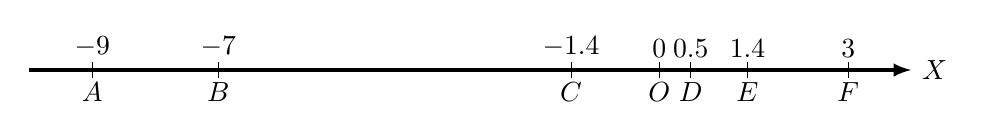
\begin{tikzpicture}[xscale=.8,>=latex]
		
		\draw[->, very thick] (-10,0)--(4,0)node[right]{$X$};        
		
		\foreach \x/\y in {-9/A,-7/B,-1.4/C,0/O,0.5/D, 1.4/E,3/F}
		{
			\draw (\x,-.1)node[above=4pt]{$\x$}--(\x,.1)node[below=4pt]{$\y$};
		}
		\end{tikzpicture}
		\caption{}
	\end{figure}
\end{solution}

不难看出:\textbf{在数轴上,右边的点总是比左边的点所表
	示的有理数要大}.因此,比较有理数的大小,就相当于在数轴上比较表示它们的点的右、左位置关系.

\begin{ex}
	比较下列各数的大小,用“$<$”号连接,并在数轴上将
	各数用点表示出来.
	\[-4,\quad -5,\quad 3.5,\quad -3,\quad 0,\quad 2,\quad -1.5,\quad 0.5,\quad 5  \]
\end{ex}

\subsection{等式与不等式的基本性质}
\subsubsection{等式}
在我们进行有理数的各种运算中,曾经遇到过这
样用等号联结的两个算式:
\[\begin{split}
(-2)+\left(-\frac{1}{3}\right) &=-2\frac{1}{3}\\
(+0.1)+(-5.1)&=-5\\
(-7)-b&=+3,\quad \text{求$b$}    \\
(-2)\cdot x&=+4,\quad \text{求$x$}    \\
\end{split}\]

我们就把\textbf{用等号“$=$”联结起来的两个算式,叫
	做等式}.如果用大写字母$A, B$表示算式,那么,等
式的一般形式就可以表示成:
\[A=B\]

显然,我们所见过的等式中,有两种类型:一类
是无须任何条件,本来就是事实的等式,如:$5+3=
(-2)+10$;$(-3)-(-16)= 13$;$a+a=2a$等.这
样的等式,我们称为\textbf{恒等式}.

另一类是必须在某些条件下,才能成为事实的等
式,如:$x+(-2)=-6$,必须在$x=-4$的条件下,
才能成为事实;$a-b=2$,必须在$a$比$b$大2的条件
下,才是事实.等等,这样的等式,称为\textbf{条件等式}.

此外,还有一种类型,根据等式的意义,只是在
犯式上用等号连结两个算式,而实际上是根本不能承
认的事实,如:$3+5=10$,$0\cdot x=-5$等.这样的等式,
称为\textbf{矛盾等式}.

对于这些等式,有以下基本性质:

\begin{blk}{}
	\begin{enumerate}
		\item 等式两边可以对调.即:如果$A= B$,那么$B=A$.
		\item 相等的关系,可以传递.即:
		如果$A=B$,  $B=C$.那么$A=C$.
		\item 等式的两边,可以加上(或减去)同一个数.即:如果$A= B$,那么$A\pm m=B\pm m$.
		\item 等式的两边,可以乘以(或除以非零的)同
		一个数.即:如果$A=B$,那么$A\cdot m=B\cdot m$ (或$A\div m =
		B\div m$) ($m\ne 0$).
	\end{enumerate}
\end{blk}


今后,多当我们遇到有关等式的问题时,就可以利
用这些基本性质,根据需要对等式进行适当的变形,
得出新的等式.

\begin{example}
	如果$a,b$两数之间有等式关系:$a-5=b-2$,
	试比较这两个数的大小,并指出大几?
\end{example}

\begin{analyze}
	要比较$a,b$的大小,就要首先把给出
	的等式$a-5=b-2$利用等式基本性质变形为“$a, b$之
	差等于几”的形式.再根据比较大小的约定得出结
	论.
\end{analyze}

\begin{solution}
	由等式$a-5=b-2$,利用等式基本性质3,
	两边可以加上同一个数5,就变形为:
	\[a-5+5=b-2+5,\text{即 } a=b+3\]
	这时已经可以知道,$a$比$b$大3.
	
	为了应用“比较大小的约定”,还可以将等式
	$a=b+3$再进一步变形为:
	\[a-b=3\qquad \text{(由性质3,两边同减$b$)}\]
	因此,$a>b$,且$a$比$b$大3.
\end{solution}

\begin{example}
	如果已知$5a + b = 7b$,试求:$\frac{a}{b},\quad (b\ne 0)$
\end{example}

\begin{solution}
	利用等式的基本性质,可作以下变形
	
	$\because\quad 5a+b=7b$ (已知)
	
	$\therefore\quad 5a=6b$ (由性质3,两边同加$(-b)$)
	
	$\therefore\quad 5\left(\frac{a}{b}\right)=6$ (由性质4,两边同除以$b\ne 0$)
	
	$\therefore\quad \left(\frac{a}{b}\right)=\frac{6}{5}$ (由性质4,两边同乘以$\frac{1}{5}$)
	
	因此,$\frac{a}{b}=\frac{6}{5}=1\frac{1}{5}$.
\end{solution}

\begin{example}
	如果等式$-4=7+11x$成立,试求$x$.
\end{example}

\begin{solution}
	利用基本性质,将等式$-4=7+11x$进行以下
	变形,可得出等式:
	\begin{align*}
	-11&=11x  \tag{两边同减去7}\\
	-1&=x  \tag{两边同除以11}\\
	x&=-1  \tag{两边对调位置}\\
	\end{align*}
\end{solution}

\begin{ex}
	\begin{enumerate}
		\item 利用等式的基本性质,试把下列的等式进行变形,你能把
		所给的每一个等式,变形成几个等式?并注明你每次变形
		的根据.
		\[b+(-3)=1,\qquad 2x+4=5y\; (y\ne 0) \]
		\item 如果$3a+b=6+4b$,你能知道$a,b$的大小吗?并指出大
		(或小)多少?
		\item $a$是何值时,等式$7a-1\frac{1}{6}=\frac{1}{2}+5\frac{1}{3}$才能成立?
		
		\item 想一想:“如果$A=B$, $C=D$,那么$A+C=B+D$”.这
		个结论对吗?举例说明.
	\end{enumerate}   
\end{ex}

\subsubsection{不等式}
在我们进行有理数的比较时,曾经运用了大于号
“$>$”与小与号,“$<$”(统称为\textbf{不等号})的符号.例
如:$5>-7$,  $1-8<-1.4+1$,正数$a>$负数$b$等.

我们就把\textbf{用不等号“$>$”或“$<$”表示出来的关系
	式,叫做不等式}.一般地记作:$A>B$(或$B<A$).

不等式同样可以分为:\textbf{恒不等式、条件不等式和
	矛盾不等式}.例如:
\begin{itemize}
	\item $5>-7,\quad   1-3<1,\quad a^2\ge 0$都是恒不等式.
	\item $a-1 >5,\qquad x+\frac{1}{2}<-1$等,都是条件不等式.
	\item $5+ (-2)<(-5)+1,\qquad -b^2>0$等都是矛盾不
	等式.
\end{itemize}

显然,对于不等式,有以下基本性质:

\begin{blk}{不等式的基本性质}
	\begin{enumerate}
		\item 如果$A>B$,那么$B<A$
		
		就是说:不等式两边对调,不等号也应调换方向.
		
		\item 如果$A>B$, $B>C$,那么$A>C$
		
		就是说:同向不等关系也可以传递.
		
		\item 如果$A>B$,那么$A+m>B+m$
		
		就是说:不等式两边,可以同加(或减)同一个数.
		\item 如果$A>B$,且$m>0$,那么$Am>Bm$
		
		就是说:不等式两边,可以乘以一个正数.
		\item 如果$A>B$,且$m<0$,那么$Am < Bm$
		
		就是说:不等式两边乘以一个负数,不等号的方
		向要改变.
	\end{enumerate}
\end{blk}

\begin{example}
	已知不等式$5a-b>\frac{1}{2}(a+7b)$,试比较$a,b$的大小.
\end{example}


\begin{solution}
	利用不等式的基本性质,可以作以下变形:
	\begin{align*}
	\because \quad & 5a-b>\frac{1}{2}(a+7b) \tag{已知}\\
	\therefore \quad & 10a-2b>a+7b \tag{不等式两边乘以2}\\
	& 9a-2b>7b \tag{不等式两边加$(-a)$}\\
	&9a>9b  \tag{不等式两边加$2b$}\\
	\therefore \quad & a>b \tag{不等式两边同乘以$\frac{1}{9}>0$}
	\end{align*}
	因此可知,$a$大于$b$.
\end{solution}

\begin{example}
	试用不等式的基本性质,说明:
	如果有理数$a>b$,那么,$a>\frac{a+b}{2}>b$.
\end{example}

\begin{note}
	由$a>b$,可作如下变形:
	\begin{align*}
	\frac{a}{2}&>\frac{b}{2} \tag{不等式两边同乘以$\frac{1}{2}>0$}   \\
	\frac{a}{2}+\frac{a}{2}&>\frac{a}{2}+\frac{b}{2} \tag{不等式两边同加$\frac{a}{2}$}   \\ 
	\end{align*}
	所以,
	\begin{equation}
	a>\frac{a+b}{2}
	\end{equation}
	同样可以类似地说明:
	\begin{equation}
	\frac{a+b}{2}>b
	\end{equation}
	因此,由(1.6)(1.7)可得出:
	\[a>\frac{a+b}{2}>b\]
\end{note}

这个例题的事实,告诉我们:\textbf{任意两个有理数
	$a, b$之间,至少可以有一个有理数$\frac{a+b}{2}$}.也就是说,
即便是相差很小的两个有理数之间,总还有另外的有
理数.这也是有理数系区别于自然数系、整数系的一
个重要特性.我们称它为有理数的\textbf{稠密性}.

\begin{ex}
	\begin{enumerate}
		\item 已知:$4a - b>3a$,试比较$a,  b$的大小.
		\item 已知:$\frac{x}{4}-1$是一个正数,$x$应取什么样的数才行?
		\item 如果$a<b$,试说明:$\frac{a-b}{10}<0$.
		\item 想一想:如果“$A>B$, $C>D$, 那么$A+C>B+D$”的结
		论对吗?举例说明.
		\item 再想想:“如果$A>B$, $C<D$, 那么$A- C>B-D$”对吗?
		举例说明.
	\end{enumerate}
\end{ex}        

\section*{习题1.4}
\addcontentsline{toc}{subsection}{习题1.4}

\begin{enumerate}
	\item 利用运算通性,计算下列各题:
	\begin{enumerate}
		\item $-1\frac{2}{3}\x \left(0.5-\frac{2}{3}\right)\div 1\frac{1}{9}$
		\item $2^3\x 5\frac{3}{5}\div (-2)\x\left(-\frac{5}{14}\right)\x \left[-1\frac{1}{2}+\left(-\frac{1}{2}\right)^2-\left(-\frac{1}{2}\right)^3\right]$
		\item $(-a)^{2n}\cdot (-a)^{2m+1}+(-1)^{2n-1}\cdot a+(-1)^{2m}a$
		\item $\frac{16^{n-2}\cdot 4^n}{8^{2n}}-\frac{5^{2n+4}\cdot 2^n}{5^{2n+3}\cdot 2^{n-3}}$
	\end{enumerate}
	
	\item 试用运算通性,说明:
	\[(a+b)^2=a^2+2ab+b^2,\qquad (a+b)\cdot (a-b)=a^2-b^2 \]
	\item 比较下列各组数的大小,并用不等号连接起来:
	\begin{enumerate}
		\item $0$ 与$-0.0001$,\quad $0.0001$ 与$-1981$,\quad $-1981$ 与$-1990$ 
		\item $-1\frac{2}{3}$ 与$-1\frac{5}{8}$,\quad $-\frac{1}{4}$ 与$100$与$-\frac{1}{7}$,\quad $\frac{4}{5}$ 与$-0.1$与$\frac{5}{4}$
		\item  $-\frac{1}{2}$ 与$0.5$与 $-2.1$ 与$0$,\quad $5\frac{1}{2}$ 与$-2\frac{1}{2}$与 $4$ 与$-\frac{1}{4}$ 
	\end{enumerate}
	
	\item 将下列各数用不等号连接起来,并画在数轴上:
	\begin{enumerate}
		\item $-\frac{1}{2},\quad  0.5 ,\quad -2.1  ,\quad 0  ,\quad -5  ,\quad  4\frac{1}{2} ,\quad 3  $
		\item $3,\quad  -5 ,\quad 5\frac{1}{2}  ,\quad  -2\frac{1}{2} ,\quad  -4 ,\quad  4 ,\quad  0 ,\quad  -3 $
	\end{enumerate}
	
	\item  在有理数$-7\frac{1}{3}$与$+5$之间(包括这两个数),找出符
	合下列条件的数:
	\begin{enumerate}
		\item 最大的有理数,最小的整数,
		\item 所有的自然数及它们的相反数.
	\end{enumerate}
	
	\item  在下列等式的变形中,试说明应用了等式的什么样基本
	性质?怎样变的?
	\begin{enumerate}
		\item $a=b\quad \Rightarrow\quad a-3=b-3$
		\item $ 5a=b  \quad \Rightarrow\quad  a=\frac{1}{5}b $
		\item  $ ab=1,\; \text{且}b\ne 0  \quad \Rightarrow\quad  a=\frac{1}{b} $
		\item  $ \frac{10}{a}=\frac{5}{b}  \quad \Rightarrow\quad a=2b  $
		\item $ -2a=-4b+2  \quad \Rightarrow\quad  a+1=2b $
	\end{enumerate}
	
	\item 利用等式的基本性质,比较$a,b$的大小:
	\begin{multicols}{2}
		\begin{enumerate}
			\item $\frac{a}{2}=\frac{b}{2}-\frac{1}{2}$
			\item $-a+b=a-b+1$
			\item $a-b=b-a$
			\item $7a+1=-1+7b$
		\end{enumerate}
	\end{multicols}
	
	\item 利用等式性质,确定下列等式中的字母应取什么值:
	\begin{multicols}{2}
		\begin{enumerate}
			\item $\frac{x}{2}=8 $
			\item $\frac{3}{5}x=-9 $
			\item $\frac{3}{4}x=-\frac{9}{2} $
			\item $-\frac{1}{2}a=\frac{2}{7} $
			\item $-12x=-\frac{3}{2} $
			\item $-9=-\frac{3}{4}b $
			\item $m+1=8 $
			\item $n-\frac{1}{2}=\frac{1}{3} $
			\item $\frac{28}{a}=-4\quad (a\ne 0) $
			\item $|x|-1=4 $
			\item $3x-7=2 $
			\item $5(x+2)=\frac{1}{2} $
		\end{enumerate}
	\end{multicols}
	
	\item 利用不等式的基本性质,比较$a, b$的大小:
	\[a-\frac{1}{2}>\frac{1}{2}+b,\qquad a-0.1>0.1+2a-b \]
	
	\item 说明在有理数$a, b$之间,一定有一个有理数$\frac{a+2b}{3}$
\end{enumerate}

\section*{本章内容要点}

一、复习和总结了小学算术中所学的数(自然
数,零及正分数)和四则运算,并进一步明确了自然
数的意义,系统说明了运算中的普遍性质(通性)这
就是:加法交换、结合律;乘法交换、结合律;分配
律及0、1的运算特性,还引进了乘方运算和指数运
算律:

乘方运算:相同因数的连乘积.
\[a^n=\underbrace{a\cdot a\cdot a\cdots a}_{\text{$n$个$a$}},\qquad a^1=a \]

指数运算律及零指数的意义:
\[a^m\cdot a^n=a^{m+n},\qquad (a\cdot b)^n=a^n\cdot b^n,\qquad (a^m)^n=a^{m\cdot n} \]
\[\left(\frac{a}{b}\right)^n=\frac{a^n}{b^n}\; (b\ne 0),\qquad a^m\div a^n=a^{m-n}\; (a\ne 0,\; m\ge n),\qquad a^0=1\;(a\ne 0) \]

\vskip 2ex 

二、由相反意义的量,引进了意义相反的正数与
负数,其特征就是“合并时,可以相消或部分相消”.
特别地,$(-a) +(+a) = 0$时,$-a$与$a$叫做互为相反
的数.$+1$与$-1$是相反意义的单位.因而将数的范围
就扩大到有理数.

有理数包括正、负整数,0及正、负分数.

一切有理数,组成有理数集合,它包含了整数集
合,而整数集合又包含了自然数集合.

任一个有理数,都可以用数轴上的一个点表示出
来.

\vskip 2ex 

三、有理数的运算法则

对有理数的运算法则,我们都是在承认运算通性
(包括运算律、指数运算律,0与1的特性)仍然有
效的前提下,合理地作了规定的.
\begin{enumerate}
	\item 加法法则:设$a,  b$是正有理数.
	\[\begin{split}
	(+a)+(+b)&=+(a+b)\\
	(-a)+(-b)&=-(a+b)\\
	(+a)+(-b)&=\begin{cases}
	+(a-b) & (a>b)\\  
	-(b-a) & (a<b)\\  
	\end{cases}    \\
	(+a)+0&=0+(+a)=+a\\
	(-a)+0&=0+(-a)=-a\\
	0+0&=0
	\end{split}\]
	\item 减法法则:设$x,  y$是有理数,
	$x-y=x+(-y)$
	\item 乘法法则:设$a,  b$是正有理数,
	\[\begin{split}
	(+a)\cdot (+b)&=+ab\\
	(-a)\cdot (+b)&=(+a)\cdot (-b)=-ab\\
	(-a)\cdot (-b)&=+ab \\
	(+a)\cdot 0&=(-a)\cdot 0=0\\
	0\x 0&=0
	\end{split}\]
	
	\item 除法法则:设$x, y$是有理数,$y\ne 0$.
	\[x\div y=x\x\frac{1}{y} \]
	
	\item 乘方法则:除了有效地应用指数运算律之外,
	有理数乘方还有以下规则:
	\begin{itemize}
		\item 正数的任何次方,仍是正数.
		\item 零的非零次方,仍是零.
		\item 负数的偶次方是正数;而负数的奇次方是负
		数.
	\end{itemize}
	
\end{enumerate}




\vskip 2ex 



四、有理数系是一个运算简便易行,通行无阻的
数集.是今后讨论数量的实际问题的有力工具.有理
数的性质可以概括为:
\begin{enumerate}
	\item 运算性质(通性).
	
	四则运算封闭;加法、乘法的交换律、结合律和
	分配律成立;零、1在运算中的特性;五个指数运算
	律成立;$a^0=1,\; (a\ne 0)$.
	
	\item 有理数可以比大小.
	\begin{itemize}
		\item 当$a-b>0$时,$a>b$;
		\item  当$a-b=0$时,$a=b$;
		\item 当$a-b<0$时,$a<b$.
	\end{itemize}
	而且,有理数的大小,正好相当于在数轴上表示这些
	有理数的点的右、左位置.我们称为“有理数的有序
	性”.
	\item 有理数的稠密性:任意两个有理数之间,存在
	着很多有理数.
\end{enumerate}

\vskip 2ex 

五、等式与不等式的基本性质.


\section*{复习题一}
\addcontentsline{toc}{section}{复习题一}

\begin{enumerate}
	\item 回答问题:
	\begin{enumerate}
		\item 最小自然数是几?最小非负整数是几?
		\item 若$a$为自然数,$\frac{5}{a}$也一定是自然数吗?
		\item 任意整数$m$,都能有倒数$\frac{1}{m}$吗?
		\item 如果$x$是有理数,$x^2$一定比$x$大吗?
	\end{enumerate}
	
	\item \begin{enumerate}
		\item 如果一个三角形的一边长为$a$,这边上的高为$h$,那么,
		这个三角形的面积$S=$?
		\item 如果把以上的三角形,底边增加一倍,那么,这个三角形的面积增加多少?
	\end{enumerate}
	
	\item 用$32$, $36$, $48$去除时,都余$15$的最小正整数应该是几?
	
	\item 计算:
	\begin{enumerate}
		\item $10^{n+1}\div 10^{n-1}  ,\qquad 100^{4n+1}\div 10^{8n-1} $
		\item $27^{2n+1}\div 9^{3n-2}  ,\qquad 5^{2n+3}\cdot 5^{3n-1}\div 5^{5n+2} $
		\item $6^{n+1}\cdot 6^{n+2} \div 6^{2n-1},\qquad 12^{n+5}\cdot 12^n\div 12^{2n+1} $
	\end{enumerate}
	
	\item 在下列条件下,求$\frac{m}{n}$的值.
	\begin{multicols}{2}
		\begin{enumerate}
			\item $m=2\frac{1}{7},\quad n=4\frac{2}{3}$
			\item $m,n$为相反数
			\item $m,n$互为倒数
			\item $m=-\frac{1}{2}n$
		\end{enumerate}
	\end{multicols}
	
	\item  \begin{enumerate}
		\item $a,b$为何值时,$a^2-b^2$表示正数?表示负数?表示零?
		\item $a$为何值时,下边的算式才成立?
		\[a>-a,\qquad a^2>a,\qquad \frac{a}{|a|}=1,\qquad \frac{a}{|a|}=-1\]
		\item 由$|m|=|n|$,能得出$m=n$的结论吗?为什么?$|m|>|n|$就可以得出$m>n$的结论吗?为什么?
		\item 如果$a,b$都是非零有理数,是否一定有:$a+b\ne 0,\; a\cdot b\ne 0$呢?举例说明.
	\end{enumerate}
	
	\item 计算:
	\begin{enumerate}
		\item $\left\{\left[\frac{2}{5}+\left(-2\frac{1}{2}+1\frac{1}{4}\right)\x 1\frac{7}{25}\right]^2-\left(\frac{7}{50}-\frac{1}{10}\right)     \right\}\div\left(\frac{17}{25}-1 \frac{2}{5}\right) $
		\item $\left\{2 \frac{3}{16}-\left[4-\left(2 \frac{1}{7}-1 \frac{1}{5}\right) \times 3.5\right] \div 0.16\right\} 
		\times\left(2 \frac{23}{24}-1 \frac{49}{60}\right) $
		\item $(-1)\div \left\{\left[(+12) \times\left(-\frac{5}{8}\right)+3 \times(-0.5) \right] \times(-4)+(-6)\right\} $
		\item $5 \frac{1}{2}\left(-\frac{6}{11}\right)-\left[-0.25+(-2)^{3}\div \left(-2 \frac{2}{3}\right) \div \frac{1}{3}\right]-\left|-\left(\frac{1}{2}\right)^{2}\right|$
	\end{enumerate}
	
	\item   如果$a$表示有理数$-\frac{1}{2}$,试说明以下各算式表示什么有理数:
	\[\left(\frac{a}{2}\cdot a^2\right)^3+a^{14}\div a^5,\qquad \frac{3a-1}{a+1}  \]
	
	\item   利用等式性质,说明以下等式中的$x$应取何值:
	\[5|x|+1=21,\qquad \frac{1}{2}|x|-1=1-\frac{1}{2}|x|  \]
	
	\item  利用不等式性质,比较$x,  y$的大小:
	\begin{enumerate}
		\item $5x-\frac{1}{5}<1+5y$;
		\item $\frac{1}{2}|x|+1>2+\frac{1}{2}|y|$.(讨论)
	\end{enumerate}
	
	\item 说明以下结论:
	\begin{enumerate}
		\item 两个奇数的和或差,都是偶数.
		\item 三个连续自然数的乘积,一定能被6整除.
		\item 如果有理数$a>b$,那么就有:$a>\frac{a+3b}{4}>b$.
		\item 没有这样的奇数$a,  b$存在,使得等式$ab-a=1981$.
	\end{enumerate}
	
	
\end{enumerate}
